\documentclass[12pt]{book}
\usepackage{mathptm,times,color}
\usepackage[pdftex]{graphicx}
\usepackage{hyperref}
\usepackage{multirow}
\usepackage{rotating}

\renewcommand{\bibname}{References}

\setlength{\textwidth}{6.5in}
\setlength{\textheight}{9.0in}
\setlength{\topmargin}{0.in}
\setlength{\headheight}{0.in}
\setlength{\headsep}{0.in}
\setlength{\parindent}{0.25in}
\setlength{\oddsidemargin}{0.0in}
\setlength{\evensidemargin}{0.0in}

\begin{document}

\bibliographystyle{unsrt}

%-----------------
\newcommand{\HGLtempavg}{14} % overall averages
\newcommand{\HGLhgtavg}{21}
\newcommand{\Plumeavg}{43}
\newcommand{\Speciesavg}{22}
\newcommand{\Targfluxavg}{2}
\newcommand{\Abstargfluxavg}{22}
\newcommand{\Abstargtempavg}{20}
\newcommand{\Surfacefluxavg}{121}
\newcommand{\Surfacetempavg}{21}

\newcommand{\HGLfurnlow}{-43} % NBS furniture HGL
\newcommand{\HGLfurnhi}{31} 
\newcommand{\furntemplow}{-4}
\newcommand{\furntemphi}{31}
\newcommand{\furnhgtlow}{-43}
\newcommand{\furnhgthi}{-1}
\newcommand{\furnoxygenavg}{22}

\newcommand{\FoneAtemp}{-4} % these are for table 6.1 showing range for NBS furniture tests
\newcommand{\FoneBtemp}{-18}
\newcommand{\FsixAtemp}{31}
\newcommand{\FsixBtemp}{-16}
\newcommand{\FoneAhgt}{-1}
\newcommand{\FoneBhgt}{-8}
\newcommand{\FsixAhgt}{-8}
\newcommand{\FsixBhgt}{-43}

\newcommand{\HGLvttlow}{6} % ranges for VTT tests
\newcommand{\HGLvtthi}{10}
\newcommand{\Plumevtt}{10}

\newcommand{\Plumefmsnl}{13} % average for FM/SNL tests, not including test 21
\newcommand{\CeilingJetfmsnl}{19}

\newcommand{\OtwoIBMB}{58}
\newcommand{\COtwoIBMB}{66}

\newcommand{\Plumehighbay}{30} % average for Navy High Bay tests

\newcommand{\HGLnistnrclow}{9} % NIST/NRC test 15
\newcommand{\HGLnistnrchi}{24} % NIST/NRC test 18
\newcommand{\CeilingJetnistnrc}{5}
\newcommand{\Oxygenclosednrc}{20}
\newcommand{\Carbondioxideclosednrc}{15}
\newcommand{\Oxygenopennrc}{7}
\newcommand{\Carbondioxideopennrc}{13}


\newcommand{\nbscorrtempavg}{14} % average absolute value HGL NBS corridor tests
\newcommand{\nbscorrhgtavg}{21} 

\newcommand{\fmnbstempavg}{14} % FM/NBS absolute averages
\newcommand{\fmnbshgtavg}{21} 
\newcommand{\fmnbsOtwoavg}{54}
\newcommand{\fmnbsCOtwoavg}{22}

\newcommand{\plazatempseven}{292} % Plaza hotel 7th floor temp

%-----------------


\newcommand{\asqh}{$A_T/A\sqrt{h}$}
\newcommand{\degc}{$^{\circ}$C }
\newcommand{\degf}{$^{\circ}$F }

\newcommand{\brackets}[1]{ { \left( {#1} \right) } }

\newcommand{\superscript}[1]{\ensuremath{^{\textnormal{#1}}}}
\newcommand{\subscript}[1]{\ensuremath{_{\textnormal{#1}}}}

\newcommand{\dx}{\delta x}
\newcommand{\dy}{\delta y}
\newcommand{\dz}{\delta z}
\newcommand{\dt}{\delta t}
\newcommand{\dQ}{\dot{Q}}
\newcommand{\dm}{\dot{m}}

\newcommand{\ha}{\frac{1}{2}}
\newcommand{\ft}{\frac{4}{3}}
\newcommand{\ot}{\frac{1}{3}}
\newcommand{\fofi}{\frac{4}{5}}
\newcommand{\of}{\frac{1}{4}}
\newcommand{\twth}{\frac{2}{3}}

\newcommand{\be}{\begin{equation}}
\newcommand{\ee}{\end{equation}}

\newcommand{\RE}{\hbox{Re}}
\newcommand{\PR}{\hbox{Pr}}
\newcommand{\NU}{\hbox{Nu}}

\newcommand{\COTWO}{{\tiny \hbox{CO}_2}}
\newcommand{\OTWO}{{\tiny \hbox{O}_2}}
\newcommand{\CO}{{\tiny \hbox{CO}}}
\newcommand{\F}{{\tiny \hbox{F}}}
\newcommand{\rb}[1]{\raisebox{1.5ex}[0pt]{#1}}

\pagestyle{empty}

\begin{minipage}[t][9in][s]{6.5in}

\huge
\flushright{NIST Special Publication 1086}
\large
\flushright{December 2012 Revision}

\vspace{1in}

\Huge
\flushright{CFAST -- Consolidated Model of Fire Growth and Smoke Transport (Version 6) \\
\LARGE Software Development and Model Evaluation Guide }

\vspace{.5in}

\large
\flushright{
Richard D. Peacock \\
Paul A. Reneke }

\vspace{.5in}

\normalsize
\flushright{http://dx.doi.org/10.6028/NIST.SP.1086}

\vfill

\center{\includegraphics[width=5.5in]{FIGURES/nistident}}

\end{minipage}

\newpage

\hspace{5in}

\newpage

\begin{minipage}[t][9in][s]{6.5in}

\huge
\flushright{NIST Special Publication 1086}

\vspace{1.in}

\Huge
\flushright{CFAST -- Consolidated Model of Fire Growth and Smoke Transport (Version 6) \\
\LARGE Software Development and Model Evaluation Guide }

\vspace{.5in}

\normalsize
\flushright{
Richard D. Peacock \\
Paul A. Reneke \\
{\em Fire Research Division} \\
{\em Building and Fire Research Laboratory} 
 }
 
 \vspace{.5in}
 
\flushright{http://dx.doi.org/10.6028/NIST.SP.1086}

\vspace{.25in}

\flushright{\today \\
$SVN Repository$~$Revision: 600 $}


\vfill

\flushright{\includegraphics[width=1in]{FIGURES/doc} }

\small
\flushright{U.S. Department of Commerce \\
{\em Rebecca Blank, Acting Secretary} \\
\hspace{1in} \\
National Institute of Standards and Technology \\
{\em Patrick D. Gallagher, Under Secretary of Commerce for Standards and Technology and Director} }

\end{minipage}




\newpage

\frontmatter

\pagestyle{plain}

\chapter{Disclaimer}

The U. S. Department of Commerce makes no warranty, expressed or implied, to users of 
CFAST and associated computer programs, and accepts no responsibility for its use.  Users of 
CFAST assume sole responsibility under Federal law for determining the appropriateness of its 
use in any particular application; for any conclusions drawn from the results of its use; and for 
any actions taken or not taken as a result of analyses performed using these tools. 
CFAST is intended for use only by those competent in the field of fire safety and is intended 
only to supplement the informed judgment of a qualified user. The software package is a 
computer model which may or may not have predictive value when applied to a specific set of 
factual circumstances. Lack of accurate predictions by the model could lead to erroneous 
conclusions with regard to fire safety. All results should be evaluated by an informed user.

\chapter{Intent and Use}

The algorithms, procedures, and computer programs described in this report constitute a 
methodology for predicting some of the consequences resulting from a prescribed fire.  They 
have been compiled from the best knowledge and understanding currently available, but have 
important limitations that must be understood and considered by the user.  The program is 
intended for use by persons competent in the field of fire safety and with some familiarity with 
personal computers. It is intended as an aid in the fire safety decision-making process.

\chapter{Preface}

This supplement to the CFAST Technical Reference Guide provides details of the software development process for CFAST and accompanying experimental evaluation of the model. It is based in part on the ``Standard Guide for Evaluating the Predictive Capability of Deterministic Fire Models,'' ASTM~E~1355~\cite{ASTM:E1355}. ASTM~E~1355 defines {\em model evaluation} as ``the process of quantifying the accuracy of chosen results from a model when applied for a specific use.'' The model evaluation process consists of two main components: verification and validation. {\em Verification} is a process to check the correctness of the solution of the governing equations. Verification does not imply that the governing equations are appropriate; only that the equations are being solved correctly. {\em Validation} is a process to determine the appropriateness of the governing equations as a mathematical model of the physical phenomena of interest. Typically, validation involves comparing model results with experimental measurement. Differences that cannot be explained in terms of numerical errors in the model or uncertainty in the measurements are attributed to the assumptions and simplifications of the physical model.

Evaluation is critical to establishing both the acceptable uses and limitations of a model. Throughout its development, CFAST has undergone various forms of evaluation, both at the National Institute of Standards and Technology and beyond. This Supplement provides a survey of validation work conducted to date to evaluate CFAST. Documentation of CFAST Verification is contained in the CFAST Technical Reference Guide~\cite{CFAST_Tech_Guide_6}.

\chapter{Acknowledgments}

\label{acksection}

Continuing support for CFAST is via internal funding at the National Institute of Standards and Technology (NIST). In addition, support is provided by other agencies of the U.S. Federal Government, most notably the Nuclear Regulatory Commission (NRC) Office of Research and the U.S. Department of Energy. The U.S. NRC Office of Research has funded key validation experiments, the preparation
of the CFAST manuals, and the continuing development of sub-models that are of importance in the area of nuclear power plant safety. Special thanks to Mark Salley and Jason Dreisbach for their efforts and support. Support to refine the software development and quality assurance process for CFAST has been provided by the U.S. Department of Energy (DOE). The assistance of Subir Sen and Debra Sparkman in understanding DOE software quality assurance programs and the application of the process to CFAST is gratefully acknowledged.  Thanks are also due to Allan Coutts, Washington Safety Management Solutions for his insight into the application of fire models to nuclear safety applications and detailed review of the CFAST document updates for DOE.

For the NIST/NRC tests, Alex Maranghides was in charge of the Large Fire Laboratory at NIST where these tests were conducted, and helped to design the experiments. Thanks also to technicians Laurean Delauter, Jay McElroy, and Jack Lee who constructed and conducted these validation experiments at NIST. Steve Nowlen at Sandia National Laboratories provided data, documentation and further information for the NRC-sponsored experiments referred to in this document and the "FM/SNL Test Series" (Factory Mutual and Sandia National Laboratories conducted these experiments). Finally, thanks to VTT, Finland, for their contribution of experimental data, referred to in this document as the ``VTT Large Hall Experiments.''

\tableofcontents

\listoffigures

\listoftables

\mainmatter

\chapter{Overview}

\section{History}

Analytical models for predicting fire behavior have been evolving since the 1960s. Over the
past decade, the completeness of the models has grown considerably. In the beginning, the focus
of these efforts was to describe in mathematical language the various phenomena which were
observed in fire growth and spread. These separate representations have typically described only
a small part of a fire. However, when combined they can create a complex computational model
that can predict the expected course of a fire.

Once a mathematical representation of the underlying physics has been developed, the conservation
equations can be re-cast into predictive equations for temperature, smoke and gas
concentration and other parameters of interest, and solved numerically.
The equations are usually in the form of differential equations. A complete set of equations can
describe the conditions produced by the fire at a given time in a specified volume of air.
Referred to as a control volume, the model assumes that the predicted conditions within this
volume are uniform at any time. Thus, the control volume has one temperature, smoke density,
gas concentration, etc. Different models divide the building into different numbers of control
volumes depending on the desired level of detail. The most common fire model, known as a
zone model, generally uses two control volumes to describe a compartment � an upper layer and
a lower layer. In the compartment with the fire, additional control volumes for the fire plume or
the ceiling jet may be included to improve the accuracy of the prediction (see figure \ref{fig:Zone_Terms}).

\begin{figure}
\begin{center}
\includegraphics[width=4.0in]{FIGURES/Overview/Zone_Terms}\\
\end{center}
\caption{Zone Model Terms.}
 \label{fig:Zone_Terms}
\end{figure}

This two-layer approach has evolved from observation of such layering in real-scale fire experiments.  Hot gases collect at the ceiling and fill the compartment from the top.  While these experiments show some variation in conditions within the layer, these are small compared to the differences between the layers.  Thus, the zone model can produce a fairly realistic simulation under many common and important conditions.

Other types of models include network models and field models.  Network models use one control volume per compartment and are used to predict conditions in spaces far removed from the fire compartment where temperatures are near ambient and layering does not occur.  The field model goes to the other extreme, dividing the compartment into thousands or millions of control volumes.  Such models can predict the variation in conditions within the layers, but typically require far longer run times than zone models.  They are used when a highly detailed prediction of the flow itself is of interest.

\section{Model Evaluation}

The process of model evaluation is critical to establishing both the acceptable uses and limitations of fire models. It is not possible to evaluate a model in total; instead, available guides such as ASTM E1355 \cite{ASTM:E1355} are intended to provide a methodology for evaluating the predictive capabilities for a specific use . Validation for one application or scenario does not imply validation for different scenarios. Several alternatives are provided for performing the evaluation process including comparison of predictions against standard fire tests, full-scale fire experiments, field experience, published literature, or previously evaluated models.

The use of fire models currently extends beyond the fire research laboratory and into the engineering, fire service and legal communities. Sufficient evaluation of fire models is necessary to ensure that those using the models can judge the adequacy of the scientific and technical basis for the models, select models appropriate for a desired use, and understand the level of confidence which can be placed on the results predicted by the models. Adequate evaluation will help prevent the unintentional misuse of fire models. Verification is a process to check the correctness of the solution of the governing equations.  Verification does not imply that the governing equations are appropriate; only that the equations are being implemented and solved correctly. Validation is a process to determine the appropriateness of the governing equations as a mathematical model of the physical phenomena of interest.  Typically, validation involves comparing model results with experimental measurement.  Differences that cannot be explained by numerical errors in the model or uncertainty in the experiments are attributed to the assumptions and simplifications of the physical model. These terms are used together to perform a model assessment. The more general term, �model assessment,� encompasses both verification and validation of a computer model.

In general, this document follows the ASTM E1355 \cite{ASTM:E1355} guide for model assessment and provides a model assessment for the zone fire model CFAST.  The guide provides four areas of evaluation for predictive fire models:

\begin{itemize}
\item Defining the model and scenarios for which the evaluation is to be conducted (chapter 2),
\item Assessing the appropriateness of the theoretical basis and assumptions used in the model (chapter 3),
\item Assessing the mathematical and numerical robustness of the model (chapter 4), and
\item Quantifying the uncertainty and accuracy of the model results in predicting the course of events in similar fire scenarios (chapters 5 and 6).
\end{itemize}

\chapter{Software Quality Assurance}

This chapter describes the processes used during the development and deployment of the Consolidated Fire and Smoke Transport model (CFAST).  This software quality assurance (SQA) plan is intended to guide the planning for modifications to the model, provide required reviews for both software and associated documentation of the model, define testing to be conducted prior to the release of an updated model, describe problem reporting and resolution procedures, and ensure all records, source code, and released software is kept available for the life of the code.  While this memorandum and many of our practices follow the IEEE standard for software quality assurance, IEEE 730-2002 \cite{IEEE:730}, other standards have been followed as well.  Most notably, ASTM 1355-05, �Standard Guide for Evaluating the Predictive Capability of Deterministic Fire Models� \cite{ASTM:E1355} has been used extensively to guide the documentation, verification, and validation of the model.

CFAST is intended for use only by those competent in the field of fire safety and is intended only to supplement the informed judgment of the qualified user. The software package is a computer model which has limitations based on the way it is used, and the data used for calculations. All results should be evaluated by a qualified user.

The SQA process and requirements outlined in this chapter apply specifically to the CFAST and is focused on ensuring the quality of the numerical predictions of the model.  The user interface that may be used to develop input for the model is included in this process to insure that changes to the model are reflected in the user interface and in the data files created by the user interface for use by the model.  Of course, users must ensure that the input files developed for the simulations accurately reflect the desired model inputs, whether developed using the supplied user interface, another third-party interface, or manually input with a spreadsheet or text editor program.  Documentation of these inputs is included as part of the model documentation outlined below.

\section{Relevant Publications}

To accompany the model and simplify its use, NIST has developed a Technical Reference Guide \cite{CFAST_Tech_Guide_6} and a User's Guide \cite{CFAST_Users_Guide_6} and this Software and Validation Guide.  The Technical Reference Guide describes the underlying physical principles and summarizes sensitivity analysis, model validation, and model limitations consistent with ASTM E 1355 \cite{ASTM:E1355}.  The User�s Guide describes how to use the model.  

The U.S. Nuclear Regulatory Commission has published a verification and validation study of five selected fire models commonly used in support of risk-informed and performance-based fire protection at nuclear power plants \cite{NRCNUREG1824_CFAST}. In addition to an extensive study of the CFAST model, the report compares the output of several other models ranging from simple hand calculations to more complex CFD codes such as the Fire Dynamics Simulator (FDS) developed by NIST.

While this document and many of our practices make extensive use of ASTM 1355, �Standard Guide for Evaluating the Predictive Capability of Deterministic Fire Models� \cite{ASTM:E1355} to guide the documentation, verification, and validation of the model, other standards have been followed as well.  Most notably, our software quality assurance processes were guided by the IEEE standard for software quality assurance, IEEE 730-2002 \cite{IEEE:730}.

In addition, numerous related documents available at http://cfast.nist.gov provide a wealth of information concerning including earlier versions of the model and its user interface. Software quality assurance (SQA) plan is intended to guide the planning for modifications to the model, provide required reviews for both software and associated documentation of the model, define testing to be conducted prior to the release of an updated model, describe problem reporting and resolution procedures, and ensure all records, source code, and ensure released software is kept available for the life of the code.  

\section{Model Management}

CFAST is developed and maintained by the Building and Fire Research Laboratory (BFRL) at the National Institute of Standards and Technology (NIST). Like all projects at BFRL, a designated project leader is responsible for directing and prioritizing model development, error correction, and preparation of documentation for the model development.  The organization chart in Figure \ref{figOrgChart} provides a graphical representation of the software quality organization structure for CFAST

\begin{figure}
\begin{center}
\includegraphics[width=6.5in]{FIGURES/OrgChart.pdf}\\
\end{center}
\caption{CFAST SQA Organization Structure.}
 \label{figOrgChart}
\end{figure}

Review and approval of software and documentation is part of the standard review process for any report or other product developed by NIST. A minimum of five reviews are required prior to release of reports or software, including two independent technical peer reviews, two technical and management reviews at the technical workgroup and division level, and a policy review at the NIST-wide level.  This review is documented and recorded on the NIST standard form NIST 114 along with official approval notification provided to the primary author of the product.

CFAST is distributed exclusively through a NIST website dedicated to the CFAST model (http://cfast.nist.gov).  Content of the website is the responsibility of the CFAST project leader and the BFRL webmaster. Additions and changes to the website are made only with the approval of the CFAST project leader after any required NIST reviews.

\section{SQA Documentation}

The released version of CFAST is documented by three primary publications, the Technical Reference Guide\cite{CFAST_Tech_Guide_6}, the User�s Guide \cite{CFAST_Users_Guide_6}, and this Software and Model Evaluation Guide. The documents apply to the newest version of the model available on the NIST website. The Technical Reference Guide describes the underlying physical principles, provides a review of model verification and validation efforts by NIST and others, and describes the limitations of the model.  The User's Guide describes how to use the model, includes a detailed description of the model inputs and outputs, and provides a process to ensure the correct installation of the model. There are also documents archived on the website that are applicable to older versions of both the model and user interface.

During development of new or corrected features for the model, the following documents are developed:

\begin{itemize}
\item {\em Software Requirements and Design Specifications:}  This is an internal memorandum that documents the intended function of a new or enhanced feature, describes its implementation in sufficient detail to allow an independent review of the feature, and identifies any new or existing testing and validation required prior to acceptance of the feature in a release version of the model.  This document forms the basis for necessary changes to the technical reference guide and user�s guide for the model once the new feature is ready for general release. As defined in IEEE 730-2002 \cite{IEEE:730}, this document includes the software requirements specification, software design description, and software verification and validation plan. The level of detail in this document depends on the complexity of the change to the model. 

\item {\em Software Validation and Testing Results:}  This is an internal memorandum that demonstrates the use of the new feature through appropriate test cases and describes validation and verification tests performed to ensure the new feature is implemented properly without unexpected changes in other features. This document forms the basis for the model verification and validation documentation included as part of this Software and Experimental Validation guide. As defined in IEEE 730-2002 \cite{IEEE:730}, this document includes the software verification and validation report. The level of detail in this document depends on the complexity of the change to the model.
\end{itemize}

Both of these documents are reviewed internally to NIST by group staff not directly involved with model development. In addition, the NIST review process documents the review and approval of released versions of the model as described above.

Source code for released versions of the model is maintained with version control software that allows tracking of specific changes to the model from version to version.   Each version of the model released includes a unique version number that identifies the major and minor version numbers of the release as well as the date of release. Differences with prior versions are documented and provided as part of the release and on the CFAST website so that users can ascertain what effect these changes will have on prior calculations.

\section{Standards, Practices, Conventions, and Metrics}

Prior to final implementation of a new feature or change, a review of the proposed modification is conducted by a developer who is not involved in the modification.  This review includes review and concurrence of the software requirements and design specification as well as more detailed review of code changes as the complexity of the modification requires. Review and acceptance of the software requirements and design specification by interested project sponsors or users may be included as appropriate. Name and date of approval and/or review is noted electronically in the document.

Review of the testing and validation report is also conducted by a developer who is not involved in the modification prior to proposed model release. Any significant changes in model output (typically a change greater than 1 \% of a given output) should be explained based on changes to the code as a result of a new feature.  Name and date of approval and/or review is noted electronically in the document.

\section{Software Reviews}

Software reviews are outlined as part of the standard practices described above.  The standard NIST review process includes review of software and documentation prior to any report or product release by NIST.

\section{Model Testing}

Individual testing of model algorithms are made by the developers during any revision of the model. Often, this testing forms the basis for any new standard test cases included with future model releases. System release testing of the model prior to release includes the following:

\begin{itemize}
\item Examination of results of test cases specific to any model modifications made as appropriate.  Comparison with analytic solutions to simplified problems is desirable when available.

\item Examination of results of standard test cases included with the release version of the model. Any changes in the output from prior versions is explained (and documented in the software testing and validation results report) by modifications made to the model.

\item For major new releases of the model, a complete suite of test cases should be compared to those from previous versions of the model.  At a minimum this includes the set of validation exercises described in NUREG 1824 \cite{NRCNUREG1824}, but may include additional example cases or validation exercises as appropriate.
\end{itemize}

\section{Problem Reporting and Resolution}

NIST maintains an e-mail address specifically for inquiries and problem reporting for the CFAST model (cfast@nist.gov).  These e-mails are directed to the CFAST project leader for response and resolution as appropriate.  Inquiries and responses are catalogued and retained by the project leader.

NIST has developed an automated reporting and resolution tracking website for use with the CFAST model to facilitate tracking and cataloging of inquires, problems, and model enhancements / revisions. This is included as part of the CFAST website at http://cfast.nist.gov

\section{Tools, Techniques, and Methodologies}

NIST will use an automated comparison tool (under development) to compare CFAST predictions between different versions of the model and with experimental data to simplify testing and validation for the CFAST model.

\section{Media Control}

Release versions of the CFAST model are available exclusively on the CFAST specific website maintained by BFRL. This website is included in NIST�s automated backup and recovery system for computer systems organization wide.

Development versions of the model are maintained by the CFAST project leader.  All software and documents are included in NIST�s automated backup and recovery system for computer systems organization wide.

Both of these computer systems are available only to specified personnel, including the CFAST project leader and BFRL webmaster.

\section{Supplier Control}

CFAST is entirely a product of BFRL / NIST and as such does not include any commercial software libraries. The differential equation solver used by CFAST, DASSL, is a publicly available software package.  Full source code for the solver as used by CFAST is maintained under version control with the rest of the model code.

BFRL currently uses Microsoft Visual Studio 2005 and Intel Visual Fortran 10.1 for development\footnote{Certain commercial entities, equipment, or materials may be identified in this document 
in order to describe an experimental procedure or concept adequately. Such identification 
is not intended to imply recommendation or endorsement by the National Institute of 
Standards and Technology, nor is it intended to imply that the entities, materials, or 
equipment are necessarily the best available for the purpose.}.  Prior to any change to a different development system, a full test suite of test cases must be compared to verify consistent operation of the model and model results.

\section{Records Collection, Maintenance, and Retention}

All software, documentation, and SQA documents are retained by the CFAST project leader, typically in electronic form. Software and documentation is also maintained and archived on the NIST CFAST website as part of the version control software for the model. 

BFRL management approval is required prior to destruction of old or out-of-date records. Records are typically maintained for a minimum of 25 years.

\section{Training}

No specific training is identified for use of this SQAP.  Details of training requirements for use of the model included in the CFAST user�s guide is applicable to developers of the model as well.

{\section{Risk Management}

The primary risk management tool for software developed and released by NIST is the official NIST review process for software, documents, and other products of NIST. Official approval is required prior to release of the model for general use.



\chapter{Software Structure and Verification}

The mathematical and numerical robustness of a deterministic computer model depends upon
three issues: the code must be transparent so that it can be understood and modified by visual
inspection; it must be possible to check and verify the coding implementation (perhaps with automated tools); and there must be a
method for checking the correctness of the solution, at least for asymptotic (steady state)
solutions (numerical stability and agreement with known solutions).

The terms {\em verification} and {\em validation} are often used interchangeably to mean the process of checking the
accuracy of a numerical model. For many, this entails comparing model predictions with experimental measurements. However,
there is now a fairly broad-based consensus that comparing model and experiment is largely what is considered {\em validation}. So what is
{\em verification}? ASTM~E~1355~\cite{ASTM:E1355}, ``Standard Guide for
Evaluating the Predictive Capability of Deterministic Fire Models,'' defines verification as
\begin{quote}
The process of determining that the implementation of a calculation method accurately
represents the developer's conceptual description of the calculation method and the solution to the calculation method.
\end{quote}
and it defines validation as
\begin{quote}
The process of determining the degree to which a calculation method is an accurate representation of the real world
from the perspective of the intended uses of the calculation method.
\end{quote}
Simply put, verification is a check of the math; validation is a check of the physics. If the model predictions closely match
the results of experiments, using whatever metric is appropriate, it is assumed by most that the model suitably describes, via
its mathematical equations, what is happening. It is also assumed that the solution of these equations must be correct. So why do
we need to perform model verification? Why not just skip to validation and be done with it? The reason is that rarely do model and
measurement agree so well in all applications that anyone would just accept its results unquestionably. Because there is
inevitably differences between model and experiment, we need to know if these differences are due to limitations or errors in
the numerical solution, or the physical sub-models, or both.

Whereas model validation consists mainly of comparing predictions with measurements, as documented later in this guide, 
model verification consists of a much broader range of activities, from checking the computer program
itself to comparing calculations to analytical (exact) solutions to understanding the impact on model outputs from a range of different model inputs.

In order to understand the meaning model verification, it is also  necessary to understand the
means by which the numerical routines are structured. In this chapter, details of the
implementation of the model are presented, including the tests used to assess the numerical
aspects of the model. These include:

\begin{itemize}
\item the structure of the model, including the major routines implementing the various
physical phenomena included in the model,
\item the organization of data initialization and data input used by the model,
\item the structure of data used to formulate the differential equations solved by the model,
\item a summary of the main control routines in the model that are used to control all input and
output, initialize the model and solve the appropriate differential equation set for the
problem to be solved,
\item the means by which the computer code is checked for consistency and correctness,
\item analysis of the numerical implementation for stability and error propagation, and
\item comparison of the results of the system model with simple analytical or numerical
solutions.
\item a series of reference test cases used to evaluate the impact of model changes to the full range of model outputs.
\end{itemize}

\section{Structure of the Numerical Routines}

A methodology which is critical to verification of the model is the schema used to incorporate
physical phenomena. This is the subroutine structure discussed below. The method for
incorporating new phenomena and ensuring the correctness of the code was adopted as part of
the consolidation of CCFM and FAST. This consolidation occurred in 1990 and has resulted in a
more transparent, transportable and verifiable numerical model. This transparency is crucial to a
verifiable and robust numerical implementation of the predictive model as discussed in the
sections on code checking and numerical analysis.

The model can be split into distinct parts. There are routines for reading data, calculating results
and reporting the results to a file or printer. The major routines for performing these functions
are identified in figure \ref{figCFASTStructure}. These physical interface routines link the CFAST model to the actual routines which calculate quantities such as mass or energy flow at one particular point in time for a given environment.

\begin{figure}[\figoptions{b}]
\begin{center}
\includegraphics[width=4.4444in]{FIGURES/Structure}\\
\end{center}
\caption[Subroutine structure for the CFAST model]{Subroutine structure for the CFAST model showing major routines and calling structure.}
 \label{figCFASTStructure}
\end{figure}

The routines SOLVE, RESID and DASSL are the key to understanding how the physical
equations are solved. SOLVE is the control program that oversees the general solution of the
problem. It invokes the differential equation solver DASSL \cite{DASSL} which in turn calls RESID to
solve the transport equations. Given a solution at time t, what is the solution at time t plus a
small increment of time, $\dt$? The differential equations are of the form

\begin{eqnarray}
   \frac{{dy}}{{dx}} &=& f(y,t) \label{eqdiffeqform}  \\
    y(t_0 ) &=& y_0 \nonumber
\end{eqnarray}

where $y$ is a vector representing pressure, layer height, mass and such, and $f$ is a vector function that represents changes in these values with respect to time. The term $y_0$ is an initial condition at
the initial time $t_0$. The time increment is determined dynamically by the program to ensure convergence of the solution at $t + \Delta t$. The subroutine RESID computes the right hand side of eq \ref{eqdiffeqform} and returns a set of residuals of that calculation to be compared to the values expected by DASSL. DASSL then checks for convergence. Once DASSL reaches an error limit (defined as convergence of the equations) for the solution at $t + \Delta t$, SOLVE then advances the solution of species concentration, wall temperature profiles, and mechanical ventilation for the same time interval.
Note that there are several distinct time scales that are involved in the solution of this type of
problem. The fastest will be chemical kinetics. In CFAST, chemical reactions are assume to be instantaneous so we ignore the impact of chemical kinetics.  The next larger time scale is that associated with the flow field. These are the equations which are cast into the form of ordinary differential equations. Then there is the time scale for mechanical ventilation, and finally, heat conduction through objects.

Chemical kinetic times are typically on the order of milliseconds. The transport time scale are
on the order of 0.1 s. The mechanical ventilation and conduction time scales are typically
several seconds, or even longer. The time step is dynamically adjusted to a value appropriate for
the solution of the currently defined equation set. In addition to allowing a more correct solution
to the pressure equation, very large time steps are possible if the problem being solved
approaches steady-state.

\section{Numerical Tests}

CFAST is designed to use 64-bit precision for real number calculations to minimize the effects of numerical error.

The differential and algebraic equation solver (called DASSL) has been tested for a variety of differential equations and is widely used and accepted \cite{DASSL}.  The radiation and conduction routines have also been tested against known solutions for asymptotic results \cite{Forney_radiation}.

Coupling between the physical algorithms of the model and the differential equation solver also works to ensure numerical accuracy by dynamically adjusting the time step used by the model to advance the solutions of the equation set. Solution tolerances are set to require solution of the model equations within one part in $10{^6}$. This ensures that the error attributable to numerical solution is far less than that associated with the model assumptions.

\section{Code Checking}
Two standard programs have been used to check the CFAST model structure and language.  Specifically, FLINT and LINT have been applied to the entire model to verify the correctness of the interface, undefined or incorrectly defined (or used) variables and constants, and completeness of loops and threads.

The CFAST code has also been checked by compiling and running the model on a variety of computer platforms.  Because FORTRAN and C are implemented differently for various computers, this represents both a numerical check as well as a syntactic check.  CFAST has been compiled for Sun (Solaris), SGI (Irix), Microsoft Windows-based PCs (Lahey, Digital, and Intel FORTRAN), and Concurrent computer platforms.  Within the precision afforded by the various hardware implementations, the model outputs are identical on the different platforms. \footnote{Typically an error limit of one part in $10^6$ which is the limit set for the differential equation solver in the solution of the CFAST equations}

The CFAST Technical Reference Guide \cite{CFAST_Tech_Guide_6} contains a detailed description of the CFAST subroutine structure and interactions between the subroutines.

\section{Comparison with Analytical Solutions}

Certain CFAST sub-models address phenomena that have analytical solutions, for example, one dimensional heat conduction through a solid or pressure increase in a sealed or slightly leaky compartment as a result of a fire or fan.  The developers of CFAST use analytical solutions to test sub-models to verify the correctness of the coding of the model as part of the development. This section provides an overview of the verification testing conducted with each change of the model to verify the basic underlying principles of the model, the mass and energy balances.

For most of the examples presented in this chapter, the same basic geometry is used, a single 5 m x 5 m x 5m compartment.  Depending on the exact simulation, additional details will be added to verify individual model results.  To begin, the simplest example is simply a compartment set at uniform ambient conditions with no ventilation, fires, or additional modeled features.  With no added mass or energy to the system, conditions are expected to remain at the initial ambient. Figure \ref{fig:Ambient_Conditions_Test} shows the simulated conditions for this simple test.

\begin{figure}
\begin{tabular*}{\textwidth}{l@{\extracolsep{\fill}}r}
\includegraphics[width=3.0in]{FIGURES/Verification/Ambient_Temperature} &
\includegraphics[width=3.0in]{FIGURES/Verification/Ambient_Pressure}
\end{tabular*}
\caption{Ambient conditions for test case with no fire, no vents, and non-conducting surfaces. Initial conditions set to 20 \degc. CFAST verification file Base.in.} \label{fig:Ambient_Conditions_Test}
\end{figure}

As a simple test of the mass and energy balance, consider the base case with the addition of a fixed amount of air (injected through a mechanical vent.  The vent is set to deliver 0.1 m$^3$/s into the compartment for 10 s. After this, the vent is closed.  Over the 10 s period, an additional 1 m$^3$ of air at ambient temperature is added.  Since CFAST, by default, closes vent over a 1 s time period, an additional 0.05 m$^3$ is also added. With a compartment volume of 125~m$^3$ at 20 \degc, the initial mass of air is 150.5 kg or 5.195 moles. With the added mass, the final mass of air in the compartment is 151.7 kg or 5.239 moles. From the CFAST output, the final temperature of the compartment rises slightly due to the pressure increase to 20.98 \degc. From the idela gas law, the expected pressure rise can be calculated as

\begin{eqnarray}
   \frac{P_i V_i}{N_i R T_i} &=&  \frac{P_f V_f}{N_f R T_f} \label{eq:Added_Mass}  \\
   P_f &=& \frac{P_i N_f  T_f}{N_i T_i}  \nonumber \\
  P_f &=& \frac{101300 \cdot 5.239 \cdot 294.13}{5.195 \cdot 293.15} \nonumber \\
  &=& 102491.3 \text{\ Pa} \nonumber
\end{eqnarray}

or a pressure rise of 1191.3 Pa, matching the calculated CFAST output of 1191.3 Pa to within 0.002~\%. Figure \ref{fig:Added_Mass_Test} shows the simulated conditions for this test.

\begin{figure}
\begin{tabular*}{\textwidth}{l@{\extracolsep{\fill}}r}
\includegraphics[width=3.0in]{FIGURES/Verification/Ambient_Temperature_Added_Mass} &
\includegraphics[width=3.0in]{FIGURES/Verification/Ambient_Pressure_Added_Mass}
\end{tabular*}
\caption{Ambient conditions for test case with no fire and non-conducting surfaces, with a mechanical ventilation system injecting 0.1~m$^3$/s of air into the compartment for 10 s. CFAST verification file Added\_Mass.in.} \label{fig:Added_Mass_Test}
\end{figure}

A similar example can be tested when the temperature of the base case compartment is raised from an initial condition of 20 \degc to 25 \degc. With conducting compartment surfaecs, the interior compartment temeprature is expected to equilibrate to the exterior. From the ideal gas law, the pressure rise can be calculated as

\begin{eqnarray}
   \frac{P_i V_i}{N_i R T_i} &=&  \frac{P_f V_f}{N_f R T_f} \label{eq:Temperature_Equilibrium}  \\
   P_f &=& T_f\frac{P_i}{T_i}  \nonumber \\
  P_f &=& 298.15 \frac{101300}{293.15} \nonumber \\
  &=& 103027.78 \text{\ Pa} \nonumber
\end{eqnarray}

or a pressure rise of 1727.78, matching the output from CFAST.  Figure \ref{fig:Temperature_Equilibrium} shows the simulated conditions for this test.

\begin{figure}[h]
\begin{tabular*}{\textwidth}{l@{\extracolsep{\fill}}r}
\includegraphics[width=3.0in]{FIGURES/Verification/Temperature_Equilibrium_Test} &
\includegraphics[width=3.0in]{FIGURES/Verification/Pressure_Change_Temperature_Equilibrium_Test}
\end{tabular*}
\caption{Ambient conditions for test case with no fire and Gypsum board surfaces, with interal initial temperature of 20~\degc and external initial temperature of 25~\degc. CFAST verification file basic\_tempequilib.in.} \label{fig:Temperature_Equilibrium}
\end{figure}

The same test can be repeated with all surfaces turned off.  With the absence of conductive surfaces, compartment conditions are not expected to change. Figure \ref{fig:Different_Ambients_Nonconducting}  shows the simulated conditions for the test case.

\begin{figure}[h]
\begin{tabular*}{\textwidth}{l@{\extracolsep{\fill}}r}
\includegraphics[width=3.0in]{FIGURES/Verification/Temperature_Equilibrium_Walls_Off} &
\includegraphics[width=3.0in]{FIGURES/Verification/Pressure_Change_Temperature_Equilibrium_Test_With_Walls_Off}
\end{tabular*}
\caption{Ambient conditions for test case with no ventilation and non-conducting surfaces.  Exterior conditions set to 25 \degc.  CFAST verification file basic\_tempequilib\_wallsoff.in.} 
\label{fig:Different_Ambients_Nonconducting}
\end{figure}

A model examining heat added to a system can be demonstrated with a test case containing a 10~s, 100 kW fire.  With non-conducting surfaces and no ventilation, the heat released from the fire can be determined since $Q=m c_p \Delta T$.  Using the CFAST generated final layer height of 3.26 m, the volume of the upper layer is calculated to be 43.451 m$^3$ and the lower layer is 81.549 m$3$.  Densities and specific heats are obtained using the temperature of each layer.  With this information the air mass of the upper layer is 49.62 kg and the lower layer air mass is 97.44 kg.  The heat added to the system can be calculated as

\begin{eqnarray}
Q &=& m c_p \Delta T \nonumber \\
Q_{upper} &=& 49.62 \cdot 1.142 (308.912 - 273.15) \nonumber \\
Q_{upper} &=& 786.25 \text{\ kJ} \nonumber \\
Q_{lower} &=& 97.44 \cdot 1.195 (295.268 - 273.15) \\
Q_{lower} &=& 207.251 \text{\ kJ} \nonumber \\
Q_{total} &=& 993.497 \text{\ kJ} \nonumber
\end{eqnarray}

or a total heat release of 993.497 kJ, or 99.35 kW over 10 s, a 0.65~\% relative difference from the CFAST input of 100 kW.The difference comes from the enrgy used to raise the pyrolyzing fuel to its ignition temperature. Figure \ref{fig:Analytical_Heat_Release_Rate} shows the simulated conditions for this test.

\begin{figure}[h]
\begin{center}
\includegraphics[width=3.0in]{FIGURES/Verification/Analytical_Heat_Release_Rate}
\caption{Heat release rate conditions for test case with a 10 s, 100 kW fire.  CFAST verification file 100kW\_fire.in.}
\label{fig:Analytical_Heat_Release_Rate}
\end{center}
\end{figure}

\section{Simple Reference Cases}

In addition to the comparisons of test cases with analytical solutions discussed in the previous section, we have included a number of simple test cases intended to demonstrate the impact of individual model features.  While these are too complex to provide analytical solutions, many can be estimated with simpler engineering calculations.  Together, these form a set of simulations that can be routinely run to verify continued consistency of the calculation results as the model is further developed to insure unintended side-effects of modifications to the model are prevented.

For completeness, the first examples dupicate the simple examples in the previsou section. As in the previous section,  most of the examples presented in this section share the same basic geometry, a single 5 m x 5 m x 5 m compartment. Unless otherwise detailed, the ‘base case’ has a single window centered on the front wall that is 2 m x 1 m and has 5/8 in Gypsum Board walls and ceiling. Depending on the exact simulation, additional details will be added to verify individual model results. 

To begin, the simplest example is the base case compartment set at uniform ambient conditions with no ventilation, fires, or additional modeled features. With no added mass or energy to the system, conditions are expected to remain at the initial ambient. Figure \ref{fig:Ambient_Conditions_Reference} shows the simulated conditions for this simple test.

\begin{figure}[h]
\begin{tabular*}{\textwidth}{l@{\extracolsep{\fill}}r}
\includegraphics[width=3.0in]{FIGURES/Verification/Ambient_Temperature} &
\includegraphics[width=3.0in]{FIGURES/Verification/Ambient_Pressure}
\end{tabular*}
\caption{Ambient conditions for test case with no fire, no vents, and non-conducting surfaces. Initial conditions set to 20 \degc. CFAST verification file Base.in.} \label{fig:Ambient_Conditions_Reference}
\end{figure}

Raising the temperature of the base case compartment from an initial condition of 20~\degc to 25~\degc, as in \ref{fig:Temperature_Equilibrium} allows the temperature to equilibrate to the exterior. Figure \ref{fig:Temperature_Equilibrium_Reference} shows the simulated conditions for this test.

\begin{figure}[h]
\begin{tabular*}{\textwidth}{l@{\extracolsep{\fill}}r}
\includegraphics[width=3.0in]{FIGURES/Verification/Temperature_Equilibrium_Test} &
\includegraphics[width=3.0in]{FIGURES/Verification/Pressure_Change_Temperature_Equilibrium_Test}
\end{tabular*}
\caption{Ambient conditions for test case with no fire and Gypsum board surfaces, with interal initial temperature of 20~\degc and external initial temperature of 25~\degc. CFAST verification file basic\_tempequilib.in.} \label{fig:Temperature_Equilibrium_Reference}
\end{figure}

The same test can be repeated with all surfaces turned off.  With the absence of conductive surfaces, compartment conditions are not expected to change. Figure \ref{fig:Different_Ambients_Nonconducting_Reference}  shows the simulated conditions for the test case.

\begin{figure}[h]
\begin{tabular*}{\textwidth}{l@{\extracolsep{\fill}}r}
\includegraphics[width=3.0in]{FIGURES/Verification/Temperature_Equilibrium_Walls_Off} &
\includegraphics[width=3.0in]{FIGURES/Verification/Pressure_Change_Temperature_Equilibrium_Test_With_Walls_Off}
\end{tabular*}
\caption{Ambient conditions for test case with no ventilation and non-conducting surfaces.  Exterior conditions set to 25 \degc.  CFAST verification file basic\_tempequilib\_wallsoff.in.} 
\label{fig:Different_Ambients_Nonconducting_Reference}
\end{figure}

The compartment surfaces are then turned back on, returning to the original base case.  With exterior conditions set to 25 \degc and a window present, conditions are expected to equilibrate to those of the exterior. Figure \ref{fig:Temperature_Equilibrium_With_Window} shows the simulated conditions for the test case.


\begin{figure}[h]
\begin{tabular*}{\textwidth}{l@{\extracolsep{\fill}}r}
\includegraphics[width=3.0in]{FIGURES/Verification/Temperature_Equilibrium_Test_With_Window} &
\includegraphics[width=3.0in]{FIGURES/Verification/Pressure_Change_Temperature_Equilibrium_Test_With_Window}
\end{tabular*}
\caption{Ambient conditions for test case with no ventilation and non-conducting surfaces.  Exterior conditions set to 25 \degc.  CFAST verification file basic\_tempequilib\_window.in.} 
\label{fig:Temperature_Equilibrium_With_Window}
\end{figure}

With the exterior temperature still set to 25 \degc, the elevation is raised to 1500 m, approximately the average elevation of Idaho.  Since CFAST calculations are relative to the exterior ambient, conditions are expected to be identical to the previous examples and equilibrate to those of the exterior. Figure \ref{fig:Temperature_Equilibrium_Elevation} shows the simulated conditions for the test case.

\begin{figure}[h]
\begin{tabular*}{\textwidth}{l@{\extracolsep{\fill}}r}
\includegraphics[width=3.0in]{FIGURES/Verification/Temperature_Equilibrium_Elevation_Change} &
\includegraphics[width=3.0in]{FIGURES/Verification/Pressure_Change_Temperature_Equilibrium_Test_Elevation}
\end{tabular*}
\caption{Ambient conditions for test case with no ventilation and non-conducting surfaces.  Exterior conditions set to 25 \degc and elevation to 1500 m.  CFAST verification file basic\_tempequilib\_window\_elevation.in.} 
\label{fig:Temperature_Equilibrium_Elevation}
\end{figure}

With the exterior temperature still set to 25 \degc, the compartment dimensions are altered to 10 m x 10 m x 5 m.  Conditions are predicted to equilibrate to those of the exterior more slowly than that of the base case model. Figure \ref{fig:Temperature_Equilibrium_Bigger} shows the simulated conditions for the test case.

\begin{figure}[h]
\begin{tabular*}{\textwidth}{l@{\extracolsep{\fill}}r}
\includegraphics[width=3.0in]{FIGURES/Verification/Temperature_Equilibrium_Compartment_Dimension_Change} &
\includegraphics[width=3.0in]{FIGURES/Verification/Pressure_Change_Temperature_Equilibrium_Test_Compartment}
\end{tabular*}
\caption{Ambient conditions for test case with no ventilation and non-conducting surfaces.  Exterior conditions set to 25 \degc and compartment dimensions enlarged to 10 m x 10 m x 10 m..  CFAST verification file basic\_tempequilib\_window\_geometry.in.} 
\label{fig:Temperature_Equilibrium_Bigger}
\end{figure}

With the exterior temperature still set to 25 \degc, the wind is raised to 10 m/s.  Temperature conditions are expected to equilibrate to those of the exterior, while the pressure will remain at a constant pressure greater than zero due to wind pressure.  Figure \ref{fig:Temperature_Equilibrium_Wind_Speed} shows the simulated conditions for the test case.

\begin{figure}[h]
\begin{tabular*}{\textwidth}{l@{\extracolsep{\fill}}r}
\includegraphics[width=3.0in]{FIGURES/Verification/Temperature_Equilibrium_Wind_Speed_Change} &
\includegraphics[width=3.0in]{FIGURES/Verification/Pressure_Change_Temperature_Equilibrium_Test_Wind}
\end{tabular*}
\caption{Ambient conditions for test case with no ventilation and non-conducting surfaces.  Exterior conditions set to 25 \degc and compartment dimensions enlarged to 10 m x 10 m x 10 m..  CFAST verification file basic\_tempequilib\_window\_geometry.in.} 
\label{fig:Temperature_Equilibrium_Wind_Speed}
\end{figure}

Two identical 5 m x 5 m x 5m compartments are set next to each other.  A 1 m$^2$ mechanical vent is added on the front face of compartment one, the shared wall between compartment one and two, and the rear wall of compartment two.  The flow rate is set to 0.1 m$^3$/s or 0.12 kg/s of air.  The mass flow through each of these vents is not expected to change because the flow rate in is constant.  Figure \ref{fig: shows the simulated conditions for the test case.
\include{Survey_Chapter}
\chapter{Description of Experiments}

This chapter summarizes the range of experiments used in the current evaluation for the CFAST model. This study focused on the predicted results of the CFAST fire model and did not include an assessment of the user interface for the model.  However, all input files used for the simulations were prepared using the CFAST graphical user interface (GUI) and reviewed for correctness prior to the simulations.  The comparisons between the experiments and model predictions were characterized as semi-blind calculations, i.e., the modelers were given detailed descriptions of the test conditions, test geometry, and fire source, but did not modify model inputs from these given conditions to improve model predictions.  As such, the comparisons in this report provide an assessment of the predictive capability of the model, but not an assessment of the ability of different modelers to develop appropriate model inputs.

\section{ATF Corridors Experiments}

A series of eighteen experiments were conducted in a two-story structure with long hallways and a connecting stairway
in the large burn room of the ATF Fire Research Laboratory in Ammendale, Maryland, in 2008~\cite{Sheppard:Corridors}.
The test enclosure consisted of two 17.0~m long hallways connected by a
stairway consisting of two staircases and an intermediary landing.
There was a door at the opposite end of the first floor hallway, which was closed during all tests.
The end of the second floor hallway was open with a soffit near the ceiling.

The walls and ceilings of the test structure were constructed of 1.2~cm gypsum wallboard.
The flooring throughout the structure, including the stairwell landing floor, consisted of one layer of 1.3~cm thick cement board on one
layer of 1.9~cm thick plywood supported by wood joists. The first set of stairs, which had eight risers, led from the first floor up to the landing area.
The second set of stairs, which had nine risers, led from the landing area up to the second floor.
The stairs were constructed of 2.5~cm thick clear pine lumber. The two set of stairs were separated by an approximately 0.42~m wide gap in the middle of the stairwell.
This gap was separated from the stairs by a 0.91~m tall barrier constructed of a single piece of gypsum board.
The flue space was open to the first floor.  The flue space was separated from the second floor by a 0.9~m tall barrier constructed of gypsum board.
There was a metal exterior type door at the end of the first floor near the burner.  The door was closed during all experiments.

The fire source was a natural gas diffusion burner.  The burner surface was horizontal, square and 0.45~m on each side, its surface was 0.37~m above the floor, and it was filled with gravel.
The burner was located near the end of the first floor away from the stairs. A diagram of the test structure is displayed in Figure~\ref{ATF Drawing}.


\begin{figure}[h]
\begin{center}
\includegraphics[width=6.5in]{FIGURES/ATF_Corridors/ATF}
\end{center}
\caption{Geometry of the ATF Corridors Experiments.}
\label{ATF Drawing}
\end{figure}

\clearpage

\section{FM Four Room Including Corridor Test Series}

This data set describes a series of tests conducted in a multiple room configuration with more complex gas burner fires than the previous data set.  This study \cite{Heskestad:1986} was included because, in many ways, it is similar to the smoke movement study performed at NBS \cite{Peacock:1988}, and permits comparisons between two different laboratories. In addition, it expands upon that data set by providing larger a time-varying gas burner fires in a room-corridor configuration. Fire size was about up to 1 MW with a total volume of 200 m$^3$.

This study was performed to collect data allowing for variations in fire source, ventilation, and geometry in a multi-compartment structure, especially for situations with closed doors. This test program was carried out at Factory Mutual Research Corporation (FMRC) in West Glocester, RI, in which 60 fire experiments were conducted in a multiple-room enclosure to furnish validation data for theoretical fire models.

Figure \ref{fig:FMSummary} shows a diagram of the basic facility with indications of instrumentation location. The facility was built on the floor of FMRC's fire test building, using part of the 67 m by 76 m test building where the ceiling height is 18.3 m. The layout in figure 25 shows a burn room and two target rooms connected to a corridor. The corridor was 2.43 m wide x 18.89 m long x 2.43 m high. The burn room measured 3.63 m deep x 3.64 m wide x 2.45 m high; a sealable window opening, measuring 0.85 m square, was centered on the rear wall, 0.34 m down from the top, and a door, measuring 0.92 m by 2.05 m high, was centered on the front wall (opening to the corridor). For closed window experiments, the wood-framed calcium silicate board window cover was pressed against a bead of caulking around the steel window frame and held by drop bars positioned into slots on the outside wall.

\begin{figure}[h]
\begin{center}
\begin{tabular}{cc}
\includegraphics[width=6.0in]{FIGURES/FM_NBS/FMSummary}\\
\end{tabular}
\end{center}
\caption{Overview of the {F}actory {M}utual Four Room test series.}
 \label{fig:FMSummary}
\end{figure}

Room 3, located opposite the burn room, measured 3.65 m deep x 3.64 m wide x 2.45 m high; a door, measuring 0.88 m by 2.02 m high, was centered on the front wall (opening to the corridor). Room 4, located at the opposite end of the corridor, measured 3.65 m deep x 3.65 m wide x 2.43 m high and had a 0.88 m by 2.02 m high door centered on the front wall (opening to the corridor); an observation alcove, measuring 1.28 m by 0.86 m by 1.99 m high, was located in the front corner of room 4. Each room was equipped with a 102~mm inside diameter vent tube with a 61 mm inside diameter orifice meter and thermocouple, with option of exhaust fan (tube centered 0.27 m from the floor and 0.17 m from the closest parallel wall). An inlet vent (0.29 m$^2$) used with exhaust fans was centered 0.43 m above the floor at the end of the corridor between the burn room and room 3. When not in use, the inlet vent was sealed with a gypsum board cover taped in place.

The target room doors were commercial fire doors (wood-faced composite doors with calcium silicate cores, 14 h rated) mounted on 16 gage steel frames. The burn room door was fabricated from 12.7 mm calcium silicate, mounted in a steel frame lined with calcium silicate. Details of the doors and the spacings (cracks) are given in the original reference \cite{Heskestad:1986}. 

Gypsum wallboard, 12.7 mm thick, on wood studs was used throughout the experimental facility. In addition, the walls and ceiling of the burn room were overlaid with calcium silicate, also 12.7 mm thick, to harden against repeated fire exposure. The existing concrete floor of the test building was used.

Two types of fire sources were used: 1) steady propylene fires at 56 kW on a 0.30 m diameter sand burner and 522 kW on a 0.91 m diameter burner and 2) propylene fires on the 0.91 m diameter burner programmed under computer control to grow with the square of time, exceeding 1 MW in 1, 2, 4, or 8 min.

The 0.91 m diameter, 0.58 in high propylene burner was used for most of the tests. Its design consisted of a 12 gage steel container with a gas distributor near the bottom, filled with gravel to a 67 percent height, where there was wire mesh screen, and coarse sand to the full height of the burner. The 0.30 m diameter burner was a scaled-down version of similar design.

\section{FM / SNL Test Series}

The Factory Mutual and Sandia National Laboratories (FM/SNL) Test Series was a series of 25 fire tests conducted in 1985 for the NRC by Factory Mutual Research Corporation (FMRC), under the direction of Sandia National Laboratories (SNL).  The primary purpose of these tests was to provide data with which to validate computer models for various types of NPP compartments.  The experiments were conducted in an enclosure measuring 18 m x 12 m x 6 m, constructed at the FMRC fire test facility in Rhode Island.  Figure \ref{fig:FMSNL_Detailed} shows detailed schematic drawings of the compartment from various perspectives.  The FM/SNL test series is described in detail, including the types and locations of measurement devices, as well as some results in References \cite{Nowlen:1987, Sandia:1989}.  Six of
the experiments were conducted with a full-scale control room mock-up in place. Parameters varied
during the experiments included fire intensity, enclosure ventilation rate, and fire location.
The current guide uses data from nineteen experiments (Tests 1-17, 21, and 22).
In these tests,  propylene gas burners, heptane pools, and methanol pools were used as fire sources.
Table~\ref{FM_SNL_Matrix} lists the test parameters.

The following information was provided by the test director,
Steve Nowlen of Sandia National Laboratory. In particular, Tests 4, 5, and 21 were given extra attention.
\begin{description}
\item[Heat Release Rate:] The HRR was determined using oxygen consumption calorimetry in the exhaust stack with
a correction applied for the carbon dioxide in the upper layer of the compartment. The
uncertainty of the fuel mass flow was not documented. Several tests selected for this study had
the same target peak heat release rate of 516~kW following a 4~min ``t-squared'' growth
profile. The test report contains time histories of the measured HRR, for which the average,
sustained HRR following the ramp up for Tests 4, 5, and 21 have been estimated as 510~kW, 480~kW, and 470~kW, respectively.
Once reached, the peak HRR was maintained essentially constant
during a steady-burn period of 6~min in Tests~4 and 5, and 16~min in Test~21. Note that in Test 21, Nowlen reports a
``significant'' loss of effluent from the exhaust hood that could lead to an under-estimate of the HRR towards the end of the experiment.
\item[Radiative Fraction:] The radiative fraction was not measured during the experiment, but
in this study it is assumed to equal 0.35, which is typical for a smoky hydrocarbons.
It was further assumed that the radiative fraction was about the same in
Test~21 as the other tests, as fuel burning must have occurred outside of the electrical cabinet in
which the burner was placed.
\item[Measurements:] Four types of measurements were conducted during the FM/SNL test series that are used in the
current model evaluation study, including the HGL temperature and depth, and the ceiling jet and
plume temperatures. Aspirated thermocouples (TCs) were used to make all of the temperature
measurements. Generally, aspirated TC measurements are preferable to bare-bead TC measurements,
as systematic radiative exchange measurement error is reduced.
\item[HGL Depth and Temperature:] Data from all of the vertical TC trees were used when reducing
the HGL height and temperature. For the majority of the tests, Sectors 1, 2, and 3 were used,
all weighted evenly. For Tests 21 and 22, Sectors 1 and 3 were used, evenly weighted. Sector 2 was
partially within the fire plume.
\end{description}

\begin{table}[h!]
\caption{Summary of FM/SNL Experiments.}
\begin{center}
\begin{tabular}{|c|c|c|c|c|c|c|}
\hline
Test    &  Fuel             & Nominal Peak  & Fire          & Ventilation       & Room                  & Used in  \\
No.     &  Type             & HRR (kW)      & Position      & Rate (ach)        & Configuration         & Guide?      \\ \hline \hline
1       & Propylene Burner  &     516       & Center        & 10                & Empty                 &        Yes \\ \hline
2       & Propylene Burner  &     516       & Center        & 10                & Empty                 &        Yes \\ \hline
3       & Propylene Burner  &    2000       & Center        & 10                & Empty                 &        Yes \\ \hline
4       & Propylene Burner  &     516       & Center        & 1                 & Empty                 &        Yes \\ \hline
5       & Propylene Burner  &     516       & Center        & 10                & Empty                 &        Yes \\ \hline
6       & Heptane Pool      &     500       & Wall          & 1                 & Empty                 &        Yes \\ \hline
7       & Propylene Burner  &     516       & Center        & 1                 & Empty                 &        Yes \\ \hline
8       & Propylene Burner  &    1000       & Center        & 1                 & Empty                 &        Yes \\ \hline
9       & Propylene Burner  &    1000       & Center        & 8                 & Empty                 &        Yes \\ \hline
10      & Heptane Pool      &    1000       & Wall          & 4.4               & Empty                 &        Yes \\ \hline
11      & Methanol Pool     &     500       & Wall          & 4.4               & Empty                 &        Yes \\ \hline
12      & Heptane Pool      &    2000       & Wall          & 4.4               & Empty                 &        Yes \\ \hline
13      & Heptane Pool      &    2000       & Wall          & 8                 & Empty                 &        Yes \\ \hline
14      & Methanol Pool     &     500       & Wall          & 1                 & Empty                 &        Yes \\ \hline
15      & Heptane Pool      &    1000       & Wall          & 1                 & Empty                 &        Yes \\ \hline
16      & Heptane Pool      &    500       & Corner        & 1                 & Empty                 &        Yes \\ \hline
17      & Heptane Pool      &    500       & Corner        & 10                & Empty                 &         No \\ \hline
18      &  PMMA Slab        &    1000       & Wall          & 1                 & Empty                 &         No \\ \hline
19      & Heptane Pool      &    1000       & Center        & 1                 & Furnished             &         No \\ \hline
20      & Heptane Pool      &    1000       & Corner        & 8                 & Furnished             &        Yes \\ \hline
21      & Propylene Burner  &     500       & Cabinet       & 1                 & Furnished             &        Yes \\ \hline
22      & Propylene Burner  &    1000       & Cabinet       & 1                 & Furnished             &         No \\ \hline
23      & Qualified Cable   &        N/A    & Cabinet       & 1                 & Furnished             &         No \\ \hline
24      & Unqualified Cable &        N/A    & Cabinet       & 1                 & Furnished             &         No \\ \hline
25      & Unqualified Cable &        N/A    & Cabinet       & 8                 & Furnished             &         No \\ \hline
\end{tabular}
\end{center}
\label{FM_SNL_Matrix}
\end{table}

\begin{figure}
\begin{center}
\includegraphics[width=8.0in, angle=90]{FIGURES/FM_SNL/FMSNL_Detailed}\\
\end{center}
\caption{Detailed plan, side, and perspective schematic drawings of the FM/SNL experimental arrangement, including the supply and exhaust ducts, and the fuel pan.}
 \label{fig:FMSNL_Detailed}
\end{figure}
 
All of the tests involved forced ventilation to simulate typical nuclear power plant installation practices.   

\begin{figure}[\figoptions{t}]
\begin{center}
\includegraphics[width=3.0in]{FIGURES/FM_SNL/FMSNL_HRR}\\
\end{center}
\caption{Prescribed (dotted line) and measured (solid line) heat release rate as a function of time during Test 21 of the FM/SNL test series}
 \label{fig:FMSNL_HRR}
\end{figure}

\section{iBMB Compartment Tests}

A series of small compartment kerosene pool fire experiments, conducted at the
Institut f\"ur Baustoffe, Massivbau und Brandschutz (iBMB) of Braunschweig University of
Technology in Germany in 2004 \cite{Klein-Helbetaling:2005}.  The results from Test 1 were
considered here.  These experiments involved relatively large fires in a relatively small (3.6 m x 3.6 m x 5.7 m) concrete enclosure. Figure  \ref{fig:iBMB_Pool_Detailed} shows plan, side and perspective schematic drawings
of the experimental arrangement, including the location of the fuel pan, which was located at the
center of the compartment.

\begin{figure}
\begin{center}
\includegraphics[width=6.5in]{FIGURES/iBMB/iBMB_Pool}\\
\end{center}
\caption{Detailed plan, side, and perspective schematic drawings of the iBMB pool fire experimental arrangement.}
 \label{fig:iBMB_Pool_Detailed}
\end{figure}
 
 Only a portion of Test 1 was selected for consideration in the present study, because a significant amount of data was lost in Test 2, and the measured ${\dQ}$  during Test 3 exhibited significant amounts of fluctuation. Five types of measurements that were conducted during the test series were used in the model evaluation reported here.  These included the HGL temperature and depth, the temperature of targets and compartment surfaces, and heat flux. In addition, figure \ref{fig:iBMB_HRR} shows the heat release rate for Test 1, which was estimated from a mass loss rate measurement.  In this calculation, the heat of combustion and the combustion efficiency were taken as 42.8 MJ/kg and 1, respectively, as suggested by Refs. \cite{NRCNUREG1824Experimental, Riese:2004}.  There were several reported difficulties in measuring the mass loss rate, including data loss due to an instrument malfunction and significant fluctuations in the measured mass loss rate. Due to these measurement issues and because the combustion efficiency was not well-characterized, the ${\dQ}$ uncertainty was assigned a relatively large expanded uncertainty of $\pm$ 25 \% \cite{NRCNUREG1824Experimental}.
 
 \begin{figure}
\begin{center}
\includegraphics[width=4.0in]{FIGURES/iBMB/iBMB_HRR}\\
\end{center}
\caption{Estimated heat release rate for the iBMB fire experiments.}
 \label{fig:iBMB_HRR}
\end{figure}

A second series of fire experiments in 2004, conducted under the International Collaborative Fire Model Project (ICFMP) involved realistically routed cable
trays inside the same concrete enclosure at iBMB \cite{Riese:2004}. The compartment was configured slightly differently with a ceiling height of 5.6 m. A schematic diagram from plan, side, and perspective views of the experimental arrangement is shown in figure \ref{fig:iBMB_Cable_Detailed}. Six types of measurements conducted during the test series were used in the evaluation conducted here, including the HGL temperature and depth, oxygen gas concentration, the temperature of targets and compartment surfaces, and heat flux.

\begin{figure}
\begin{center}
\includegraphics[width=6.5in]{FIGURES/iBMB/iBMB_Cable}\\
\end{center}
\caption{Detailed plan, side, and perspective schematic drawings of the iBMB cable fire experimental arrangement.}
 \label{fig:iBMB_Cable_Detailed}
\end{figure}

The results of four tests were
available, of which one has been used in the current study.
These tests were conducted primarily for the evaluation of cable ignition and flame spread.
The results were erratic, and no replicate experiments were performed. Given the primitive
nature of the ignition and spread algorithms within the models, it was decided that only
a qualitative analysis would be possible with the data from three of the four experiments.
However, in one experiment, the first 20 minutes involved a fairly well-characterized ethanol
pool fire burning on the opposite side of the compartment from the cable tray. This part of
the experiment has been used as part of the model evaluation.

The first part of the test consisted of preheating the cable trays in the room with a 1 m$^2$ round pan on the floor filled with ethanol (ethyl alcohol) used as the preheating source.  At 30 min, a propane gas burner was used as the fire source � this was not considered because only the first 20 min of the test was used in this validation study.  
Exhaust products were collected in an exhaust duct and the $\dQ$  was measured using the oxygen calorimetry.  For the purpose of this study, the measured $\dQ$ was used as direct input to the various fire models.  The first 20 min of data were used for the model evaluation. After 20 min, the  $\dQ$ became relatively noisy.  Figure \ref{fig:iBMB_HRR} shows the HRR. The relative combined expanded uncertainty was assigned a value of $\pm$15 \%, consistent with typical values of this parameter \cite{NRCNUREG1824Experimental}.

\section{LLNL Enclosure Tests}

Sixty-four enclosure fire tests were conducted by Lawrence Livermore National Laboratory (LLNL) in 1986 to study the effects of ventilation on enclosure fires~\cite{Foote:LLNL1986}. The test
enclosure was 6~m long, 4~m wide, and 4.5~m high. It contained a methane rock burner which was placed in the center of the space. For most of the tests the burner was placed on the
floor. The fires varied in size from 50~kW to 400~kW. The burner was 0.57~m in diameter and 0.23~m height.

The door (2.06 m high by 0.76 m wide) was closed and sealed for most tests, and air was pulled through the space at rates varying from 100 to 500~g/s. In some tests the enclosure included a plenum space, where
make-up air could be injected from above or below. The test matrix is listed in Table~\ref{LLNL_Matrix}.

\begin{table}[p]
\caption[Summary of LLNL Enclosure Experiments]{Summary of LLNL Enclosure Experiments.}
\begin{center}
\begin{tabular}{|c|c|c|c|c|c||c|c|c|c|c|c|}
\hline
Test & Room    & $h_0$ &  $\dot{Q}$ & $\dot{m}$ & $T_\infty$  &   Test & Room    & $h_0$ &  $\dot{Q}$ & $\dot{m}$ & $T_\infty$  \\              
No.  & Config. & m     &  kW        & g/s       & $^\circ$C   &   No.  & Config. & m     &  kW        & g/s       & $^\circ$C   \\ \hline \hline
1    & TL      & 0     & 200        & 0         & 23          &   33   & PH      & 0     & 100        & 200       & 23          \\ \hline              
2    & TL      & 0     & 200        & 0         & 27          &   34   & PH      & 0     & 100        & 300       & 34          \\ \hline              
3    & TL      & 0     & 400        & 0         & 27          &   35   & PH      & 0     & 100        & 400       & 22          \\ \hline              
4    & TL      & 0     & 300        & 0         & 24          &   36   & PH      & 0     & 100        & 500       & 29          \\ \hline              
5    & TL      & 0     & 50         & 0         & 28          &   37   & PH      & 0     & 200        & 100       & 20          \\ \hline              
6    & TL      & 0     & 100        & 0         & 29          &   38   & PH      & 0     & 200        & 300       & 29          \\ \hline              
7    & TL      & 0     & 100        & 0         & 35          &   39   & PH      & 0     & 250        & 100       & 18          \\ \hline              
8    & TL      & 0     & 200        & 0         & 35          &   40   & PH      & 0     & 200        & 400       & 28          \\ \hline              
9    & TL      & 0     & 200        & 500       & 33          &   41   & PH      & 0     & 150        & 100       & 20          \\ \hline              
10   & TL      & 0     & 200        & 100       & 28          &   42   & PHE     & 2     & 200        & 180       & 30          \\ \hline              
11   & TL      & 0     & 200        & 200       & 18          &   43   & PHE     & 2     & 200        & 0         & 32          \\ \hline              
12   & TL      & 0     & 200        & 300       & 21          &   44   & PHE     & 1     & 200        & 180       & 19          \\ \hline              
13   & TL      & 0     & 200        & 400       & 28          &   45   & PHE     & 1     & 200        & 0         & 30          \\ \hline              
14   & TL      & 0     & 200        & 400       & 28          &   46   & PHE     & 0.6   & 200        & 180       & 19          \\ \hline              
15   & TL      & 0     & 100        & 300       & 24          &   47   & PHE     & 0.6   & 200        & 0         & 19          \\ \hline              
16   & TL      & 0     & 200        & 300       & 21          &   48   & PHE     & 0.3   & 200        & 0         & 21          \\ \hline              
17   & PL      & 0     & 200        & 500       & 26          &   49   & PHE     & 0.3   & 200        & 180       & 26          \\ \hline              
18   & PL      & 0     & 200        & 400       & 21          &   50   & PHE     & 1     & 200        & 180       & 21          \\ \hline              
19   & PL      & 0     & 200        & 300       & 18          &   51   & PNE     & 1     & 200        & NAT       & 33          \\ \hline              
20   & PL      & 0     & 200        & 200       & 16          &   52   & PN      & 0     & 200        & NAT       & 23          \\ \hline              
21   & PL      & 0     & 200        & 100       & 23          &   53   & PHGS    & 0     & 200        & 185       & 33          \\ \hline              
22   & PH      & 0     & 200        & 190       & 30          &   54   & PHGS    & 0     & 200        & 215       & 21          \\ \hline              
23   & PH      & 0     & 200        & 215       & 28          &   55   & PN      & 0     & 100        & NAT       & 31          \\ \hline              
24   & PH      & 0     & 200        & 205       & 26          &   56   & PHGW    & 0     & 200        & 190       & 20          \\ \hline              
25   & PH      & 0     & 200        & 205       & 25          &   57   & PHGW    & 0     & 200        & 215       & 29          \\ \hline              
26   & PH      & 0     & 200        & 500       & 24          &   58   & PHX     & 0     & 200        & 190       & 18          \\ \hline              
27   & PH      & 0     & 200        & 100       & 23          &   59   & PHXE    & 1     & 200        & 190       & 24          \\ \hline              
28   & PH      & 0     & 150        & 150       & 31          &   60   & PN      & 0     & 400        & NAT       & 22          \\ \hline              
29   & PH      & 0     & 250        & 250       & 28          &   61   & TN      & 0     & 200        & NAT       & 31          \\ \hline              
30   & PH      & 0     & 250        & 300       & 34          &   62   & TN      & 0     & 400        & NAT       & 22          \\ \hline              
31   & PH      & 0     & 250        & 500       & 36          &   63   & TN      & 0     & 50         & NAT       & 28          \\ \hline              
32   & PH      & 0     & 100        & 100       & 33          &   64   & TN      & 0     & 100        & NAT       & 17          \\ \hline 
\end{tabular}
\end{center} 
\begin{tabbing}
\hspace{0.7in} \= T \hspace{0.2in}  \= full compartment     \hspace{0.8in} \= N \hspace{0.2in} \= natural ventilation (door open) \\
               \> P                 \> plenum configuration                \> X                \> 3 ft extension on inlet opening \\
               \> L                 \> low inlet duct                      \> GS               \> grate on inlet, north/south configuration \\
               \> H                 \> high inlet duct                     \> GW               \> grate on inlet, east/west configuration \\
               \> E                 \> elevated fire, $h_0$ 
\end{tabbing}       
\label{LLNL_Matrix}  
\end{table}              


\begin{figure}[\figoptions{b}]
\begin{center}
\includegraphics[width=6.5in]{FIGURES/LLNL_Enclosure/LLNL_Enclosure_Drawing}
\end{center}
\caption[Geometry of the LLNL Enclosure Experiments]{Geometry of the LLNL Enclosure Experiments.}
\label{LLNL_Enclosure_Drawing}
\end{figure}

\section{NBS Single Room Tests with Furniture}

These data describe a series of room fire tests using upholstered furniture items in a room of fixed size but with varying opening sizes and shapes \cite{Valid:Babrauskas_Flashover} conducted by the National Bureau of Standards (NBS, former name of NIST). It was selected for its well characterized and realistic fuel sources in a simple single-room geometry. In addition, the wide variation in opening size should provide challenges for current zone fire models. Peak fire size was about 2.9~MW with a total room volume of 21 m$^3$. A series of four single-room fire tests were conducted using upholstered furniture items for comparison with their free burning behavior, previously determined in a furniture calorimeter.  The experiments were conducted in a single room enclosure; ventilation to the room was provided by window openings of  varying sizes. The room was equipped with an instrumented exhaust collection system outside the window opening.  

A second similar test series also utilized a single-room fire test with furniture as the fire source \cite{Lee:1985}. It expanded upon the first data set by adding the phenomenon of wall burning. Peak fire size was about 7 MW. The room size was similar to the first test series. Figure \ref{fig:NBSFurniture} illustrates the configuration for the two test series.

\begin{figure}[\figoptions{b}]
\begin{center}
\includegraphics[width=5.0in]{FIGURES/NBS/NBSFurniture}\\
\end{center}
\caption[Plan and elevation view schematic of experimental room for NBS single room tests with furniture.]{Plan and elevation view schematic of experimental room for NBS single room tests with furniture. Note dotted lines on burning specimen indicates vertical surface for wall burning experiments.  Specimen and instrumentation placement are approximate.}
 \label{fig:NBSFurniture}
\end{figure}

\begin{figure}[\figoptions{b}]
\begin{center}
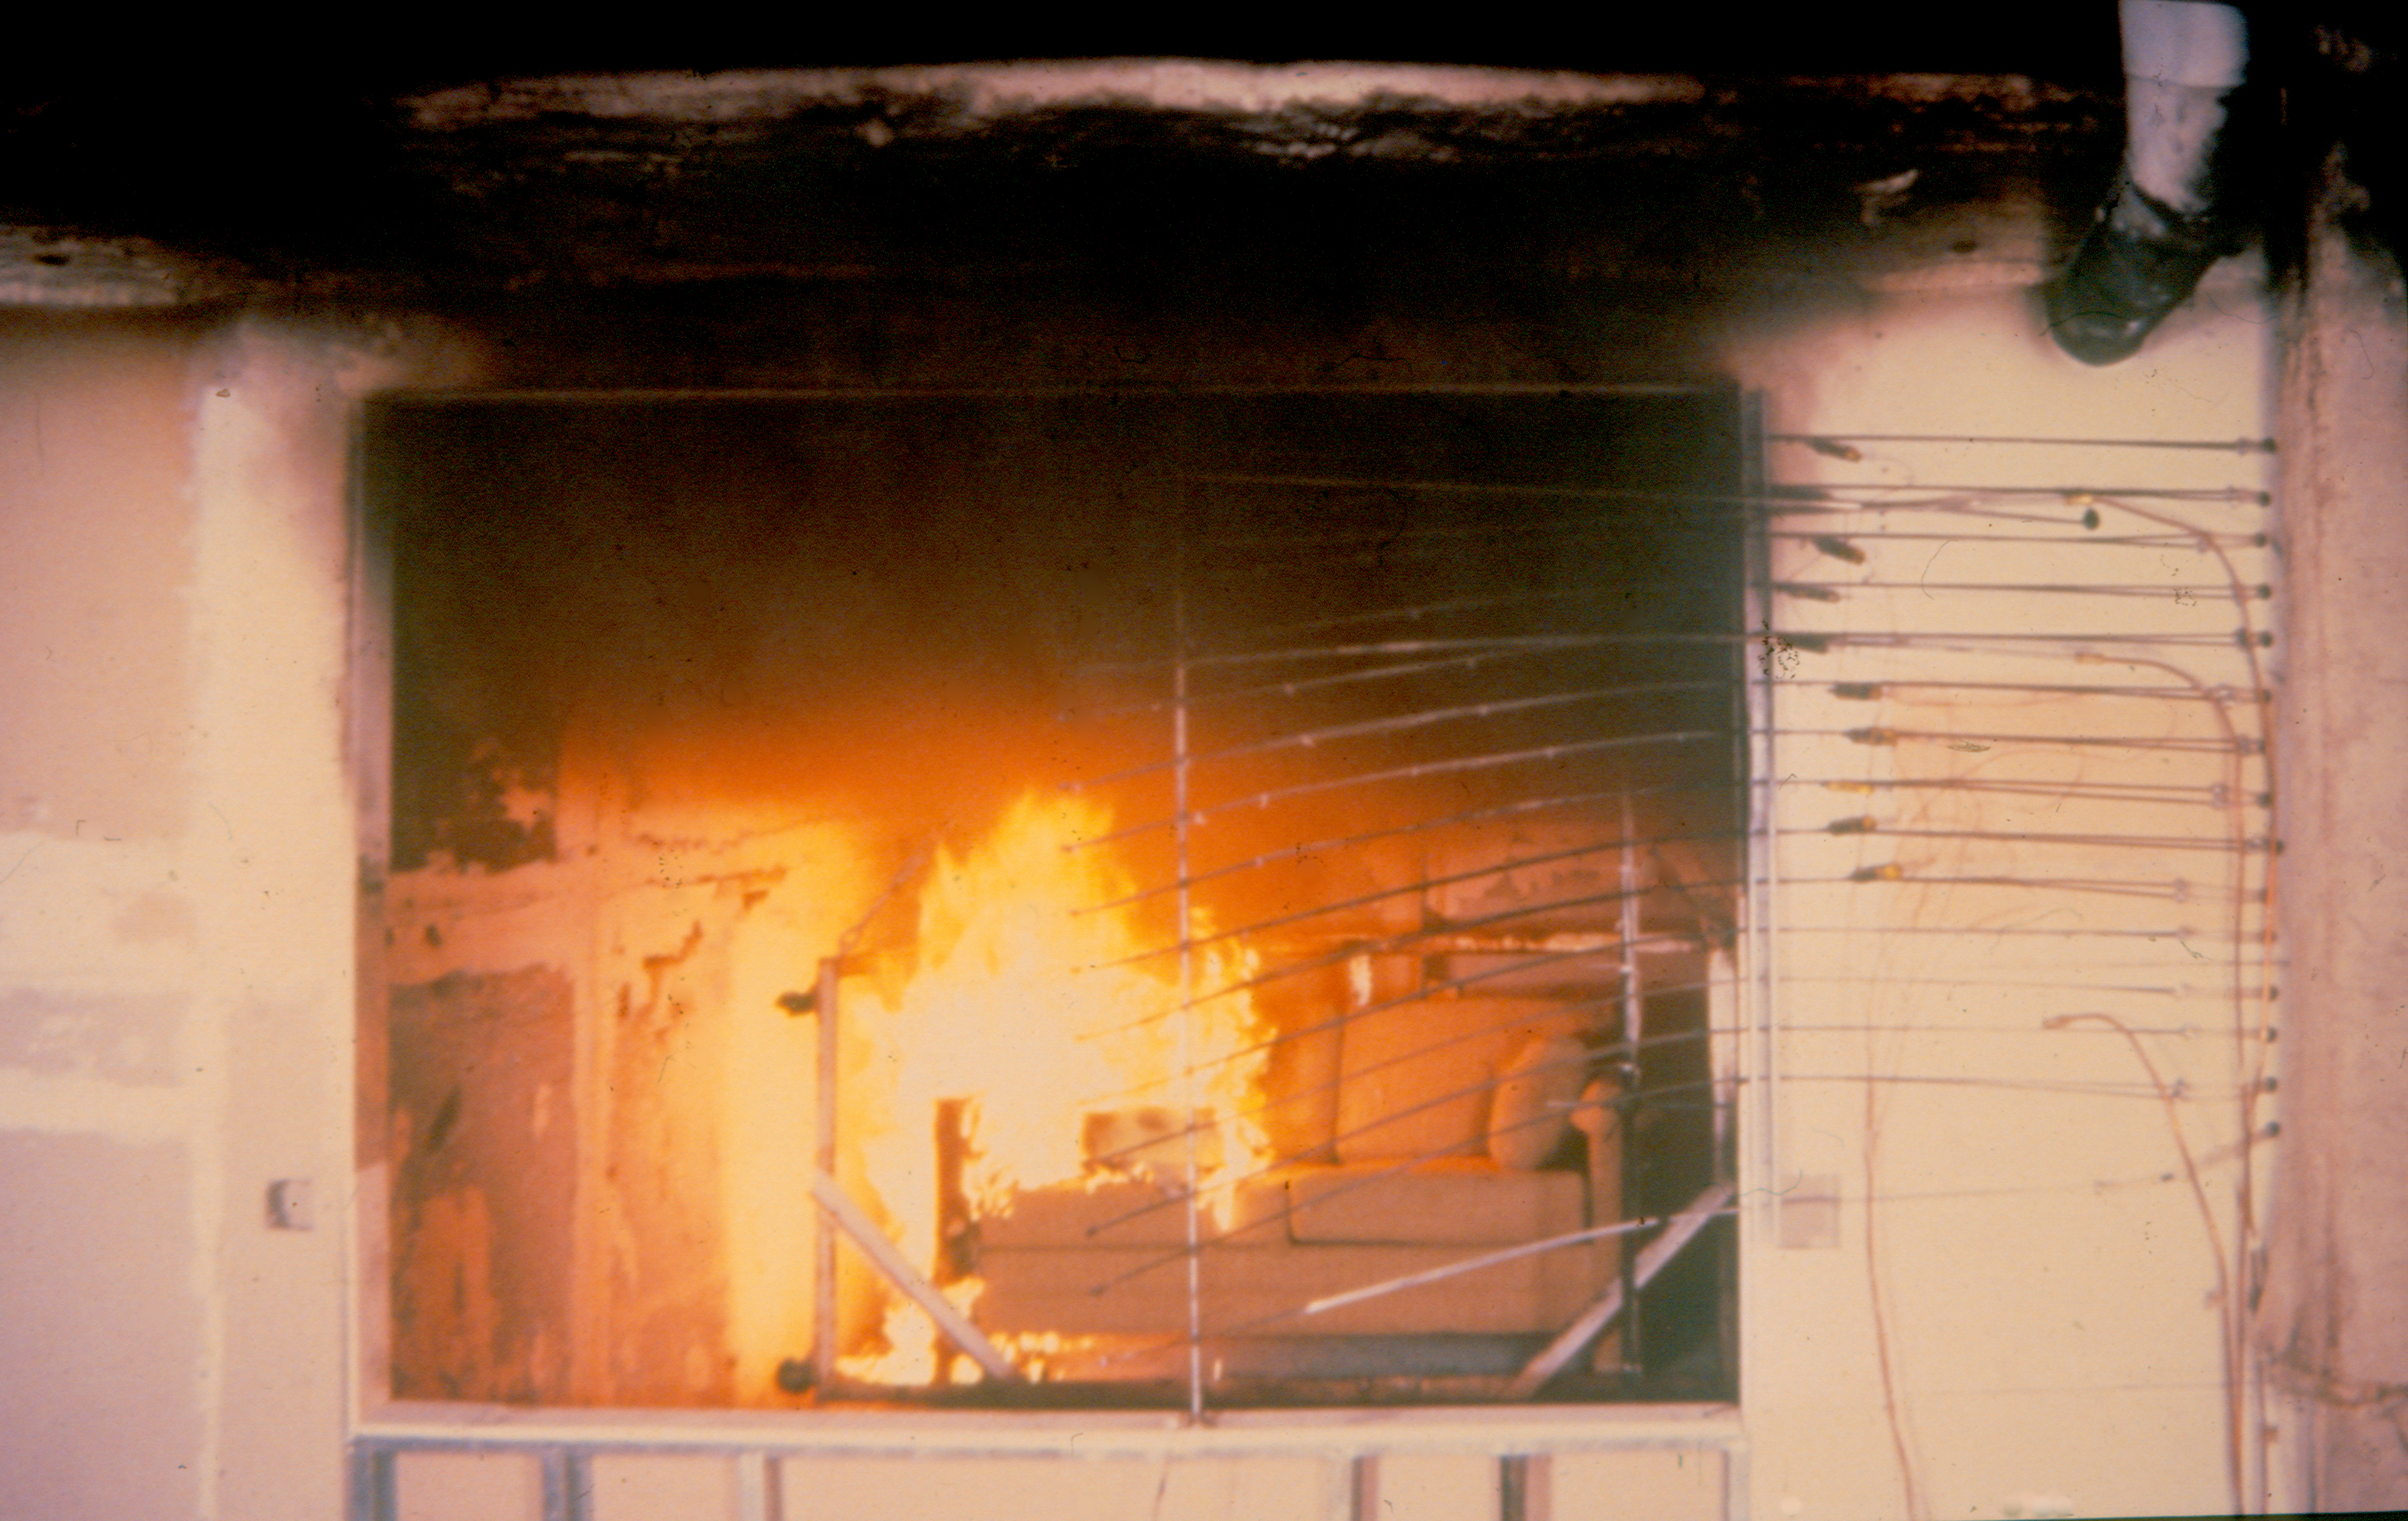
\includegraphics[width=5.0in]{FIGURES/NBS/NBS_Furniture_Test}\\
\end{center}
\caption[Burning specimen during NBS single room tests with furniture.]{Burning specimen during NBS single room tests with furniture.}
 \label{fig:NBSFurniturePix}
\end{figure}

The test furniture included a 28.3 kg armchair or a similar 40.0 kg love seat for the first test series. Both were of conventional wood frame construction and used polyurethane foam padding, made to minimum California State flammability requirements, and polyolefin fabric. A single piece of test furniture and igniting wastebasket were the only combustibles in the test room. 

For the second test series, room furnishings consisted of a 1.37 m wide x 1.91 m long x 0.53 m high double bed, a 2.39 m X 0.89 m high headboard, and 0.51 m wide x 0.41 m deep x 0.63 m high night table. Both headboard and night table were fabricated from 12.7 mm thick plywood. The bedding was comprised of two pillows, two pillow cases, two sheets, and one blanket. The pillows had a polypropylene fabric with a polyester filling. The pillow cases and sheets were polyester-cotton. The blanket was acrylic material. The bedding was left in a "slept in" condition which was duplicated to the degree possible in each test. In all of the tests, the fire was started with match flame ignition of a 0.34 kg (240 mm x 140 mm x 240 mm high) wastebasket, filled with 0.41 kg of trash, positioned adjacent to the bed.

\section{NBS Multi-Compartment Test Series}

The National Bureau of Standards (NBS, former name of NIST) Multi-Compartment Test Series consisted of 45 fire tests representing 9 different sets of conditions were conducted in a three-room suite.  The experiments were conducted in 1985 and are described in detail in reference \cite{Peacock:1988}.  The suite consisted of two relatively small rooms, connected via a relatively long corridor. Total volume of the structure was approximately 100 m$^2$. The fire source, a gas burner, was located against the rear wall of one of the small compartments as seen in Figure \ref{fig:NBS_100kW_fire} for a 100 kW fire.  Figures \ref{fig:NBS_Summary} and \ref{fig:NBS_Detailed} presents the experimental arrangement in the form of plan, side and perspective schematic drawings of the compartments. Fire tests of 100 kW, 300 kW and 500 kW were conducted. For the current  study, three 100 kW fire experiments have been used, including Test 100A from Set 1, Test 100O from Set 2, and Test 100Z from Set 4. For the NBS Multi-room series, Tests 100A, 100O and 100Z were selected for study, because they were constructively used in a previous validation study [\cite{EPRI}, and because these tests had  the steadiest values of measured heat release rate during the steady burning period. The selected data are also available in Reference \cite{EPRI}.   Reference \cite{NRCNUREG1824Experimental} provides information used as model input for simulation of the NBS tests, including information on the compartment, the fire, the ventilation, and ambient conditions. The data in the NBS data set was acquired every 10 s with a 6 s time-average.  This time-averaging interval was somewhat smaller than all of the other experimental series, which were time-averaged over a 10 s interval. 

\begin{figure}
\begin{center}
\includegraphics[width=2.0in]{FIGURES/NBS/NBS_100kW_fire}  \\
\end{center}
\caption{Photo of a 100 kW fire with the burner located against the rear wall of one of the small compartments in the NBS Multi-Compartment test Series.}
 \label{fig:NBS_100kW_fire}
\end{figure}

\begin{figure}[\figoptions{t}]
\begin{center}
\includegraphics[width=5.0in]{FIGURES/NBS/NBS_Summary}\\
\end{center}
\caption{Overview of the NBS Test Configuration.}
 \label{fig:NBS_Summary}
\end{figure}

\begin{figure}[\figoptions{t}]
\begin{center}
\includegraphics[width=8.0in, angle=90]{FIGURES/NBS/NBS_Detailed}\\
\end{center}
\caption{Plan, side and perspective schematic drawings of the NBS experimental arrangement, including the burner.}
 \label{fig:NBS_Detailed}
\end{figure}

Figures \ref{fig:NBS_HRR} show the experimentally measured $\dQ$ as a function of time during Tests 100A and 100Z, respectively, of the NBS multi-room test series, typically averaging about 100 kW.  In these two tests, for which the door was open, the $\dQ$ during the steady burning period measured via oxygen consumption calorimetry was about 110 kW $\pm$ 17 kW ($\pm$ 15 \%) \cite{NRCNUREG1824Experimental}. The combined relative expanded (2$\sigma$) uncertainty in the calorimetric  $\dQ$ is assigned a value of $\pm$~15~\%, consistent with the replicate measurements made during the experimental series and the uncertainty typical of oxygen consumption calorimetry \cite{NRCNUREG1824Experimental}. This value is also consistent with the measurement variation evident in the figures.  It was assumed that the closed door test (Test 100O) had the same $\dQ$ as the open door tests \cite{NRCNUREG1824Experimental}.

\begin{figure}[\figoptions{t}]
\begin{center}
\begin{tabular}{cc}
\includegraphics[width=3.0in]{FIGURES/NBS/NBS_HRR_100A} & \includegraphics[width=3.0in]{FIGURES/NBS/NBS_HRR_100Z}\\
\end{tabular}
\end{center}
\caption{Prescribed and measured heat release rate as a function of time during Tests 100A and 100Z of the NBS multi-room test series.}
 \label{fig:NBS_HRR}
\end{figure}

The specified or prescribed  $\dQ$ is also shown in the figures.   The mass flow of the fuel (natural gas in Test 100A, or natural gas mixed with acetylene in Tests 100O and 100Z) was not metered; rather, the effluent was captured in a hood mounted above the open door in the corridor and the   was measured using oxygen consumption calorimetry.  The manner by which the fuel flow was controlled is not documented.  In Test 100A, candles were used to increase smoke in the upper layer to promote visualization. In Tests 100O and 100Z, acetylene was used (about 20 \% by volume) to produce smoke.  In those tests, the flow of natural gas and acetylene were adjusted to obtain approximately the same $\dQ$  as in Test 100A.  The addition of acetylene increased the radiative fraction of the fire. 

For practical reasons, piped natural gas supplied by large utility companies is often used in fire experiments.  While its composition may vary from day to day, there is little change expected in the value of the radiative fraction \cite{NRCNUREG1824Experimental}. As mentioned above, natural gas was used as the fuel in Test 100A.  In Tests 100O and 100Z, acetylene was added to the natural gas to increase the smoke yield, and as a consequence, the radiative fraction increased.  The radiative fraction of natural gas has been studied previously, whereas the radiative fraction of the acetylene/natural gas mixture has not been studied. The radiative fraction for the natural gas fire was assigned a value of 0.20, whereas a value of 0.30 was assigned for the natural gas/acetylene fires \cite{NRCNUREG1824Experimental, Hamins:1991}.  

The relative combined expanded (2$\sigma$) uncertainty in this parameter was assigned a value of $\pm$~20 \% in Test 100A and $\pm$~30 \% in 100O and 100Z.  The 20 \% expanded deviation value is consistent with typical values of the deviation reported in the literature for the measured radiative fraction.  The 100O and 100Z tests had a 50 \% larger value assigned, because the effect on the radiative fraction of adding acetylene to the natural gas was not measured \cite{NRCNUREG1824Experimental}.

Measurements made during the NBS test series included gas and surface temperature, pressure, smoke and major gas species concentration, and doorway gas velocity.  Only two types of measurements conducted during the NBS test series were used in the evaluation considered here, because there was less confidence in the other measurements.  The measurements considered here were the HGL temperature and depth, in which bare bead thermocouples were used to make these measurements.  Single point measurements of temperature within the burn room were not used in the evaluation of plume or ceiling jet algorithms.  This is because, in neither instance, was the geometry consistent with the assumptions used in the model algorithms of plumes or jets. Specifically, the burner was mounted against a wall, and the room width to height ratio was less than that assumed by the various ceiling jet correlations.

\section{NIST Dunes 2000 Experiments}

A series of experiments was conducted by NIST to measure the activation time of ionization and photoelectric
smoke alarms in a residential setting~\cite{Bukowski:1}. Tests were conducted in actual homes with
representative sizes and floor plans, utilized actual furnishings and household items for fire sources,
and tested actual smoke alarms sold in retail stores at that time. Thirty-six tests were conducted in two
homes; 27 in a single-story manufactured home, and 8 in a two-story home.

Figure~\ref{NIST_Dunes_2000_Drawing} shows a diagram of the layout and instrumentation in the
manufactured home. The primary partitioning of the 84.7~m$^2$ floor plan consisted of three bedrooms:
one full bathroom, one kitchen/dining area, one living room, and two hallways. For testing, the doors
to bedroom 3 and the bathroom were always closed. The ceiling
was peaked on the long axis, reaching a height of 2.4~m. The outside walls
were approximately 2.1~m in height. The slope of the ceiling was approximately 8.4$^\circ$.

An upholstered chair, mattress, or pan of cooking oil was used as the fire source in each test.
There were three primary ignition sources: flaming, smoldering, and cooking.
The flaming ignition source used a moderate flame source to quickly ignite the fuel package.
Groups of smoke alarms were located in the room of fire origin, at least one bedroom, and
in a central location. Five stations (A-E) containing smoke alarm arrays were mounted parallel to the ceiling.

\begin{figure}[h]
\begin{center}
\includegraphics[width=6.5in]{FIGURES/NIST_Dunes_2000/NIST_Dunes_2000_Drawing}
\end{center}
\caption[Geometry of the NIST Dunes 2000 Experiments]{Geometry of the NIST Dunes 2000 Experiments.}
\label{NIST_Dunes_2000_Drawing}
\end{figure}


\section {NIST Seven-story Hotel Tests}

By far the most complex test, this data set is part of  a series of full-scale experiments conducted to evaluate zoned smoke control systems, with and without stairwell pressurization \cite{Klote:1990}.  It was conducted in a seven story hotel with multiple rooms on each floor and a stairwell connecting all floors.  This data set was chosen because it would challenge the scope of most current fire models.  Measured temperatures and pressure differences between the rooms and floors of the building are extensive and consistent.  Peak fire size was 3 MW with a total building volume of 140~000 m$^3$.

Smoke movement and the performance of smoke control systems were studied in a seven story hotel building with smoke generated from wood fires and theatrical smoke. A total of 12 single experiments were conducted under a variety of conditions: two different fire sizes; sprinklered vs non-sprinklered wood fires; zoned smoke control on or off; stairwell pressurization on or off; with and without ventilation to the outside; and open and closed doors. 

The Plaza Hotel building was a masonry structure consisting of two wings, one three stories and the other seven stories tall. The two wings were built at different times. The wings were connected to each other at only one location on each floor. The connections between the wings at each floor were sealed off, and the fires were set on the second floor of the seven-story wing, using the shorter wing as an instrumentation area. Areas of the second floor were fire hardened to minimize structural damage to the building.

\begin{figure}[\figoptions{t}]
\begin{center}
\begin{tabular}{cc}
\includegraphics[width=6.0in]{FIGURES/NIST_PLAZA/PlazaSummary}\\
\end{tabular}
\end{center}
\caption{Overview of the NIST Seven-story hotel test series including smoke control.}
 \label{fig:PlazaSummary}
\end{figure}

The smoke control systems were designed using the methods presented in the smoke control manual of the American Society of Heating, Refrigerating, and Air-Conditioning Engineers \cite{Klote:1983}, and the design analysis is discussed in detail by Klote \cite{Klote:1988}. The minimum design pressure difference was 25 Pa, meaning that the system should be able to maintain at least this value without a fire. The Plaza Hotel building had no central forced air heating, ventilating, and air-conditioning (HVAC) system, so a dedicated system of fans and ducts was installed for zoned smoke control and stairwell pressurization. The smoke control system consisted of the three 0.944 m$^3$/s centrifugal fans shown in \ref{fig:PlazaSummary}, plus another centrifugal fan (not shown) located outside and supplying 4.25 m$^3$/s of pressurization air to the stairwell at the first floor. The smoke control system is illustrated in figure \ref{fig:PlazaSummary}. All the test fires were located in the second floor smoke zone. This smoke was exhausted at about six air changes per hour. The first and second floors were pressurized at about six air changes per hour. When the stairwell pressurization system was activated, the exterior stairwell door was open. This approach is intended to minimize fluctuations due to opening and closing doors.

\section{NIST / NRC Test Series}

These experiments, sponsored by the US NRC and conducted at NIST, consisted of 15 large-scale experiments performed in June 2003. All 15 tests were included in the validation study. The experiments are documented in Ref.~\cite{Hamins:2005}. The fire sizes ranged from 350 kW to 2.2 MW in a compartment with dimensions 21.7~m by 7.1~m by 3.8~m high, designed to represent a compartment in a nuclear power plant containing power and control cables. A photo of the fire seen through the compartment doorway is shown in figure \ref{fig:NISTNRC_1MW_fire}. Figure \ref{fig:NISTNRC_Summary} shows the important features of the test hall. Figure \ref{fig:NISTNRC_Detailed} shows detailed plan, side and perspective schematic diagrams of the experimental arrangement. The walls and ceiling were covered with two layers of marinate boards, each layer 0.0125~m thick. The floor was covered with one layer of gypsum board on top of a layer of plywood. Thermo-physical and optical properties of the marinate and other materials used in the compartment are given in reference \cite{Hamins:2005}. The room had one door and a mechanical air injection and extraction system. Ventilation conditions, the fire size, and fire location were varied. Numerous measurements (approximately 350 per test) were made including gas and surface temperatures, heat fluxes and gas velocities. Detailed schematic diagrams of the experimental arrangement are shown in figure \ref{fig:NISTNRC_Detailed}. Table \ref{tab:NISTNRC_Matrix} shows the experimental conditions for all 15 tests. 

\begin{figure}[\figoptions{t}]
\begin{center}
\includegraphics[width=4.0in]{FIGURES/NIST_NRC/NISTNRC_1MW_fire}\\
\end{center}
\caption{Photograph of a 1 MW heptane fire seen through the open doorway. Photo provided by Anthony Hamins, NIST.}
 \label{fig:NISTNRC_1MW_fire}
\end{figure}

\begin{figure}[\figoptions{t}]
\begin{center}
\includegraphics[width=5.0in]{FIGURES/NIST_NRC/NISTNRC_Summary}\\
\end{center}
\caption{Cross-section View of the NIST NRC Test Configuration.}
 \label{fig:NISTNRC_Summary}
\end{figure}

\begin{figure}[\figoptions{t}]
\begin{center}
\includegraphics[width=8.0in, angle=90]{FIGURES/NIST_NRC/NISTNRC_Detailed}\\
\end{center}
\caption{Plan, side and perspective schematic drawings of the NIST NRC experimental arrangement. The fuel pan and cables B, D, F, and G (dotted lines) are also shown.}
 \label{fig:NISTNRC_Detailed}
\end{figure}

\begin{table}
\begin{center}
\caption{Test Matrix and Experimental Conditions for NIST NRC Tests}
\label{tab:NISTNRC_Matrix}
\vspace{0.1in}
\begin{tabular}{|c|c|c|c|c|c|}
\hline
Test & Nominal Peak & Cable & Fuel; Burner Location & Door & Mechanical\\
 & $\dQ$ (MW) & Type &  &  & Ventilation \\ \hline
\hline
1 & 0.35 & XPE\superscript{a} & Heptane; Center & Closed & Off \\ \hline
2 & 1 & XPE & Heptane; Center & Closed & Off \\ \hline
3 & 1 & XPE & Heptane; Center & Open & Off \\ \hline
4 & 1 & XPE & Heptane; Center & Closed & On \\ \hline
5 & 1 & XPE & Heptane; Center & Open & On \\ \hline
6 & \multicolumn{5}{|c|}{Not Conducted} \\ \hline
7 & 0.35 & PVC\superscript{b} & Heptane; Center & Closed & Off \\ \hline
8 & 1 & XPE & Heptane; Center & Closed & Off \\ \hline
9 & 1 & XPE & Heptane; Center & Open & Off \\ \hline
10 & 1 & PVC & Heptane; Center & Closed & On \\ \hline
11& \multicolumn{5}{|c|}{Not Conducted} \\ \hline
12 & \multicolumn{5}{|c|}{Not Conducted} \\ \hline
13 & 2 & XPE & Heptane; Center & Closed & Off \\ \hline
14 & 1 & XPE & Heptane; 1.8 m from N wall & Open & Off \\
 & & & on E-W centerline & & \\ \hline
15 & 1 & PVC & Heptane; 1.25 m from S wall & Open & Off \\ 
 & & & on E-W centerline & & \\ \hline
 16 & 2 & PVC & Heptane; Center & Closed & On \\ \hline
 17 & 1 & PVC & Toluene; Center & Closed & Off \\ \hline
18 & 1 & XPE & Heptane; 1.55 m from S wall & Open & Off \\
 & & & 1.50 m E of centerline & & \\ \hline 
\multicolumn{6}{l}{a - XPE cable has crosslinked polyethylene jacket insulation} \\
\multicolumn{6}{l}{b - PVC cable has a polyvinylchloride jacket insulation}
\end{tabular}  
\end{center}
\end{table}

The compartment had a 2 m by 2 m door in the middle of the west wall. Some of the tests had a closed door and no mechanical ventilation, and in those tests the measured compartment leakage was an important consideration. Reference \cite{Hamins:2005} reports leakage area based on measurements performed periodically during the test series. For the closed door tests, the leakage area used in the simulations was based on the last available measurement. It should be noted that the chronological order of the tests differed from the numerical order \cite{Hamins:2005}. 

The mechanical ventilation and exhaust was used during some test, providing about 5 air changes per hour. The supply duct was positioned on the long wall, about 2 m off the floor. An exhaust duct of equal area to the supply duct was positioned on the opposite wall at a comparable location. The flow rates through the supply and exhaust ducts were measured in detail during breaks in the testing, in the absence of a fire. During the tests, the flows were monitored with single bi-directional probes during the tests themselves.

A single nozzle was used to spray liquid hydrocarbon fuels onto a 1 m by 2 m fire pan that was about 0.02 m deep. The test plan originally called for the use of two nozzles to provide the fuel spray. Experimental observation suggested that the fire was more steady with the use of a single nozzle. In addition, it was observed that the actual extent of the liquid pool was well-approximated by a 1 m circle in the center of the pan. For safety reasons, the fuel flow was terminated when the lower-layer oxygen concentration dropped to approximately 15~\% by volume. The fuel used in 14 of the tests was heptane, while toluene was used for one test. The HRR was determined using oxygen consumption calorimetry (figure \ref{fig:NISTNRC_HRR} shows a sample heat release rate for one of the tests in the series). The recommended uncertainty values for HRR were 17~\% for all of the tests. The radiative fraction was measured in an independent study for the same fuels using the same spray burner as used in the test series \cite{Hamins:2003}. The value of the radiative fraction and its uncertainty were reported as 0.44 $\pm$ 16 \% and 0.40 $\pm$ 23 \% for heptane and toluene, respectively. Further details of the model inputs used for these simulations are included in reference \cite{NRCNUREG1824Experimental}.

\begin{figure}[\figoptions{t}]
\begin{center}
\includegraphics[width=3.0in]{FIGURES/NIST_NRC/NISTNRC_HRR}\\
\end{center}
\caption{Measured and prescribed heat release rate as a function of time during Test 3 of the NIST NRC test series}
 \label{fig:NISTNRC_HRR}
\end{figure}

\section{Steckler Compartment Experiments}

Steckler, Quintiere and Rinkinen performed a set of 55 compartment fire tests at NBS in 1979 \cite{Steckler:1982}. The compartment was 2.8~m by 2.8~m by 2.13~m high\footnote{The test report
gives the height of the compartment as 2.18~m. This is a misprint. The compartment was 2.13~m high.}, with a single door of
various widths, or alternatively a single window with various heights. A 30~cm diameter methane burner was used to generate fires with heat release rates of
31.6~kW, 62.9~kW, 105.3~kW and 158~kW. Vertical profiles of velocity and temperature were measured in the doorway, along with a single vertical profile of temperature
within the compartment.
A full description and results are reported in Reference~ \cite{Steckler:1982}. The basic test matrix is listed in Table~\ref{Steckler_Table}. Note that the
test report does not include a detailed description of the compartment. However, an internal report\footnote{ {\em Technical Research Report, Fire Induced Flows
Through Room Openings - Flow Coefficients}, Project 203005-003, Armstrong Cork Company, Lancaster, Pennsylvania, May, 1981.} by the test sponsor, Armstrong Cork Company,
reports that the compartment floor was composed of 19~mm calcium silicate board on top of 12.7~mm plywood on wood joists. The walls and ceiling consisted of
12.7~mm ceramic fiber insulation board over 0.66~mm aluminum sheet attached to wood studs.

\begin{table}[h!]
\caption{Summary of Steckler compartment experiments.}
\begin{center}
\begin{tabular}{|c|c|c|c|c||c|c|c|c|c|}
\hline
        & Opening   & Opening       &  HRR       & Burner       &       & Opening   & Opening     &  HRR         & Burner        \\
Test    & Width     & Height        & $\dot{Q}$  & Location     & Test  & Width     & Height      & $\dot{Q}$    & Location      \\
        & (m)       & (m)           & (kW)       &              &       & (m)       &  (m)        & (kW)         &                \\ \hline \hline
10      & 0.24      & 1.83          &  62.9      & Center       & 224   & 0.74      & 0.92        &  62.9         & Back Corner         \\ \hline
11      & 0.36      & 1.83          &  62.9      & Center       & 324   & 0.74      & 0.92        &  62.9         & Back Corner         \\ \hline
12      & 0.49      & 1.83          &  62.9      & Center       & 220   & 0.74      & 1.83        &  31.6         & Back Corner         \\ \hline
612     & 0.49      & 1.83          &  62.9      & Center       & 221   & 0.74      & 1.83        &  105.3        & Back Corner         \\ \hline
13      & 0.62      & 1.83          &  62.9      & Center       & 514   & 0.24      & 1.83        &  62.9         & Back Wall           \\ \hline
14      & 0.74      & 1.83          &  62.9      & Center       & 544   & 0.36      & 1.83        &  62.9         & Back Wall           \\ \hline
18      & 0.74      & 1.83          &  62.9      & Center       & 512   & 0.49      & 1.83        &  62.9         & Back Wall           \\ \hline
710     & 0.74      & 1.83          &  62.9      & Center       & 542   & 0.62      & 1.83        &  62.9         & Back Wall           \\ \hline
810     & 0.74      & 1.83          &  62.9      & Center       & 610   & 0.74      & 1.83        &  62.9         & Back Wall           \\ \hline
16      & 0.86      & 1.83          &  62.9      & Center       & 510   & 0.74      & 1.83        &  62.9         & Back Wall           \\ \hline
17      & 0.99      & 1.83          &  62.9      & Center       & 540   & 0.86      & 1.83        &  62.9         & Back Wall           \\ \hline
22      & 0.74      & 1.38          &  62.9      & Center       & 517   & 0.99      & 1.83        &  62.9         & Back Wall           \\ \hline
23      & 0.74      & 0.92          &  62.9      & Center       & 622   & 0.74      & 1.38        &  62.9         & Back Wall           \\ \hline
30      & 0.74      & 0.92          &  62.9      & Center       & 522   & 0.74      & 1.38        &  62.9         & Back Wall           \\ \hline
41      & 0.74      & 0.46          &  62.9      & Center       & 524   & 0.74      & 0.92        &  62.9         & Back Wall           \\ \hline
19      & 0.74      & 1.83          &  31.6      & Center       & 541   & 0.74      & 0.46        &  62.9         & Back Wall           \\ \hline
20      & 0.74      & 1.83          &  105.3     & Center       & 520   & 0.74      & 1.83        &  31.6         & Back Wall           \\ \hline
21      & 0.74      & 1.83          &  158.0     & Center       & 521   & 0.74      & 1.83        &  105.3        & Back Wall           \\ \hline
114     & 0.24      & 1.83          &  62.9      & Back Corner  & 513   & 0.74      & 1.83        &  158.0        & Back Wall           \\ \hline
144     & 0.36      & 1.83          &  62.9      & Back Corner  & 160   & 0.74      & 1.83        &  62.9         & Center$^*$          \\ \hline
212     & 0.49      & 1.83          &  62.9      & Back Corner  & 163   & 0.74      & 1.83        &  62.9         & Back Corner$^*$     \\ \hline
242     & 0.62      & 1.83          &  62.9      & Back Corner  & 164   & 0.74      & 1.83        &  62.9         & Back Wall$^*$       \\ \hline
410     & 0.74      & 1.83          &  62.9      & Back Corner  & 165   & 0.74      & 1.83        &  62.9         & Left Wall$^*$       \\ \hline
210     & 0.74      & 1.83          &  62.9      & Back Corner  & 162   & 0.74      & 1.83        &  62.9         & Right Wall$^*$      \\ \hline
310     & 0.74      & 1.83          &  62.9      & Back Corner  & 167   & 0.74      & 1.83        &  62.9         & Front Center$^*$    \\ \hline
240     & 0.86      & 1.83          &  62.9      & Back Corner  & 161   & 0.74      & 1.83        &  62.9         & Doorway$^*$         \\ \hline
116     & 0.99      & 1.83          &  62.9      & Back Corner  & 166   & 0.74      & 1.83        &  62.9         & Front Corner$^*$    \\ \hline
122     & 0.74      & 1.38          &  62.9      & Back Corner  &  \multicolumn{5}{r|}{$^*$ Raised burner}                   \\ \hline
\end{tabular}
\end{center}
\label{Steckler_Table}
\end{table}

\section{USN High Bay Hangar Experiments}

The U.S. Navy sponsored a series of 33 tests within two hangars examining fire detection and sprinkler activation in response to spill fires in large enclosures \cite{Gott:1997, Davis:2000}. Experiments were conducted using JP-5 and JP-8 fuels in two Navy high bay aircraft hangars located in Naval Air Stations in Barber's Point, Hawaii and Keflavik, Iceland.

The Hawaii tests were conducted in a 15~m high hangar measuring 97.8~m in length and 73.8~m in width. Of the 13 tests conducted in the facility 11 were conducted in pans ranging from .09~m$^2$ to 4.9~m$^2$ in area with heat release rates varying from 100~kW to 7.7~MW. The burner was placed in the center of the room on a scale that continuously recorded the pans weight. The facility was equipped with a number of detection devices including thermocouples, electronic smoke and spot heat detectors, projected beam smoke detectors, combination UV/IR optical flame detectors, line-type heat detectors, as well as sprinklers. Measurements were recorded at a large number of locations allowing for a through profile of compartment behavior.

It was suspected that fire plume behavior and response of detection devices in a cold building may not have been well replicated by the experiments held in the warm hangar in Hawaii. The Iceland tests were conducted under a 22~m barrel vaulted ceiling in a hangar measuring 45.7~m by 73.8~m. 22 tests in total were conducted. The majority of these tests fires burned JP-5 fuel with the remainder burning JP-8. The jet fuel fires ranged in size from .06~m$^2$ to 20.9~m$^2$ and in heat release rate from 100~kW to approximately 33~MW. The facility was equipped similarly to the Hawaii hangar.

\section{Vettori Flat Ceiling Experiments}

Vettori~\cite{Vettori:1} analyzed a series of 45 experiments conducted at NIST that were intended to compare the effects of different ceiling configurations on the activation times of quick response residential pendent sprinklers. The two ceiling configurations used consisted of an obstructed ceiling, with parallel beams 0.038~m wide by 0.24~m deep placed 0.41~m on center, and a smooth ceiling configuration, in which the beams were covered by a sheet of gypsum board.  In addition to the two ceiling configurations, there were also three fire growth rates and three burner locations used -- a total of 18 test configurations. The fire growth rate was provided by a computer controlled methane gas burner to mimic a standard t-squared fire growth rate with either a slow, medium, or fast ramp up. The burner was placed in a corner of the room, then against an adjacent wall, and then in a location removed from any wall. Measurements were taken to record sprinkler activation time, temperatures at varying heights and locations within the room, and the ceiling jet velocities at several other locations.  A diagram of the test structure is displayed in Figure~\ref{Vettori_Drawing}.

\begin{figure}[\figoptions{b}]
\begin{center}
\includegraphics[width=6.5in]{FIGURES/Vettori_Flat/Vettori_Flat_Ceiling}
\end{center}
\caption[Geometry of the Vettori Flat Ceiling compartment]{Geometry of the Vettori Flat Ceiling compartment.}
\label{Vettori_Drawing}
\end{figure}

\section{VTT Large Hall Tests}

The experiments are described in reference~\cite{Hostikka:2001}. The series consisted three unique fire scenarios with replications for a total of 8 experiments. The experiments were undertaken to study the movement of smoke in a large hall with a sloped ceiling. The tests were conducted inside the VTT Fire Test Hall, with dimensions of 19 m high by 27 m long by 14 m wide. Figure \ref{fig:VTT_cutaway} shows the important features of the test hall. Figure \ref{fig:VTT_Schematic} shows detailed plan, side and perspective schematic diagrams of the experimental arrangement. Each test involved a single heptane pool fire, ranging from 2~MW to 4~MW. Figure \ref{fig:VTT_2MW_fire} is a photo of a 2~MW fire. Four types of measurements were used in the present evaluation -- the hot gas layer temperature and depth, average flame height and the plume temperature. Three vertical arrays of thermocouples, plus two thermocouples in the plume, were compared to model simulation results. The hot gas layer temperature and height were reduced from an average of the three thermocouple arrays using a standard algorithm. The ceiling jet temperature was not considered, because the ceiling in the test hall is not flat, and the model algorithm is not appropriate for these conditions.

\begin{figure}[\figoptions{b}]
\begin{center}
\includegraphics[width=5.0in]{FIGURES/VTT/VTT_Cut_Away}\\
\end{center}
\caption{Cut-Away View of Case 2 of the VTT Large Hall Tests.}
 \label{fig:VTT_cutaway}
\end{figure}

\begin{figure}[\figoptions{b}]
\begin{center}
\includegraphics[width=8.0in, angle=90]{FIGURES/VTT/VTT_Schematic}\\
\end{center}
\caption{Plan, side and perspective schematic drawings of the experimental arrangement of the VTT large hall fire tests, including the fuel pan}
 \label{fig:VTT_Schematic}
\end{figure}

\begin{figure}[\figoptions{b}]
\begin{center}
\includegraphics[width=3.0in]{FIGURES/VTT/VTT_2MW_fire}\\
\end{center}
\caption{Photo of a 2 MW heptane fire during the VTT large hall tests. Photo provided by Simo Hostikka, VTT.}
 \label{fig:VTT_2MW_fire}
\end{figure}

The VTT test report lacks some information needed to model the experiments, so some information was based on private communications with the principal investigator, Simo Hostikka. Details used to conduct the model simulations is presented in reference \cite{NRCNUREG1824Experimental}, including information on the fire, the compartment, and the ventilation.

The walls and ceiling of the test hall consist of a 1 mm thick layer of sheet metal on top of a 5 cm layer of mineral wool. The floor was constructed of concrete. The report does not provide thermal properties of these materials. Thermophysical properties of the materials that were used in the simulations are given in table \ref{tab:VTT_Thermals}.

\begin{table}[h!]
\begin{center}
\caption{Thermophysical Properties for VTT Large Hall Tests}
\label{tab:VTT_Thermals}
\vspace{0.1in}
\begin{tabular}{|l|c|c|c|c|c|}
\hline
Material & Conductivity & Specific Heat & Density & Thickness & Emissivity\\
 & W/m$^{\circ}$C & J/kg$^{\circ}$C & kg/m$^3$ & m & \\ \hline
\hline
Steel ICFMP BE2 & 54 &        425 &       7850 &      0.001 &       0.95  \\ \hline
Concrete ICFMP BE2 &          2 &        900 &        230 &       0.15 &       0.95 \\ \hline
\end{tabular}  
\end{center}
\end{table}

In Cases 1 and 2, all doors were closed, and ventilation was restricted to leakage through the building envelope. Precise information on air infiltration during these tests is not available. The scientists who conducted the experiments recommend a leakage area of about 2~m$^2$, distributed uniformly throughout the enclosure. By contrast, in Case 3, the doors located in each end wall (Doors 1 and 2, respectively) were open to the external ambient environment. These doors are each 0.8 m wide by 4 m high, and are located such that their centers are 9.3 m from the south wall. The test hall had a single mechanical exhaust duct, located in the roof space, running along the center of the building. This duct had a circular section with a diameter of 1 m, and opened horizontally to the hall at a distance of 12 m from the floor and 10.5 m from the west wall. Mechanical exhaust ventilation was operational for Case 3, with a constant volume flow rate of 11 m$^3$/s drawn through the 1 m diameter exhaust duct. 

Each test used a single fire source with its center located 16 m from the west wall and 7.4 m from the south wall. For all tests, the fuel was heptane in a circular steel pan that was partially filled with water. The pan had a diameter of 1.17 m for Case 1 and 1.6 m for Cases 2 and 3. In each case, the fuel surface was 1 m above the floor. The trays were placed on load cells, and the HRR was calculated from the mass loss rate. For the three cases, the fuel mass loss rate was averaged from individual replicate tests. In the HRR estimation, the heat of combustion (taken as 44.6 kJ/g) and the combustion efficiency for n-heptane was used.  In this report, a combustion efficiency of 0.85 $\pm$ 0.12 (or $\pm$ 14 \%) was used for the VTT pool fire tests \cite{NRCNUREG1824Experimental}. Due to the relatively large value of the uncertainty associated with the combustion efficiency the uncertainty in HRR is dominated by the uncertainty in the combustion efficiency. Uncertainty in the mass loss rate measurement also contributed to the overall uncertainty, and the uncertainty in HRR was estimated as 15 \% \cite{NRCNUREG1824Experimental}. Figure \ref{fig:VTT_HRR} show the prescribed HRR as a function of time during Cases 1 to 3, respectively. The radiative fraction was assigned a value of 0.35 \cite{NRCNUREG1824Experimental}, similar to many smoky hydrocarbons \cite{Hamins:1991}. The relative combined expanded (2$\sigma$) uncertainty in this parameter was assigned a value of $\pm$ 20 \%, which is typical of uncertainty values reported in the literature for this parameter. Further details of the model inputs used for these simulations are included in reference \cite{NRCNUREG1824Experimental}.

\begin{figure}[p]
\begin{center}
\begin{tabular}{c}
\includegraphics[width=2.6in]{FIGURES/VTT/VTT_Case1_HRR} \\
\includegraphics[width=2.6in]{FIGURES/VTT/VTT_Case2_HRR} \\
\includegraphics[width=2.6in]{FIGURES/VTT//VTT_Case3_HRR}
\end{tabular}
\end{center}
\caption{Prescribed Heat Release Rate as a Function of Time for VTT Large Hall Tests.} \label{fig:VTT_HRR}
\end{figure}

\clearpage
\clearpage

\section{WTC Spray Burner Test Series}

As part of its investigation of the World Trade Center disaster, the Building and Fire Research Laboratory at NIST conducted several series of fire experiments to both gain insight into the
observed fire behavior and also to validate FDS for use in reconstructing the fires. The first series of experiments involved a relatively simple compartment with a liquid spray burner and
various structural elements with varying amounts of sprayed fire-resistive materials (SFRM). A diagram of the compartment is shown in figure~\ref{WTC_Drawing}.
A complete description of the experiments can be found in the NIST WTC report NCSTAR~1-5B~\cite{NIST_NCSTAR_1-5B}.
The overall enclosure was rectangular, as were the vents and most of the obstructions. The compartment walls and ceiling were made of 2.54~cm thick marinite. The manufacturer provided the thermal properties of the material used in the calculation. The density was 737~kg/m$^3$, conductivity 0.12~W/m/K. The specific heat ranged from 1.17~kJ/kg/K at 93~$^\circ$C to
1.42~kJ/kg/K at 425~$^\circ$C. This value was assumed for higher temperatures.
The steel used to construct the column and truss flanges was 0.64~cm thick.  The density of the steel was assumed to be 7,860~kg/m$^3$; its specific heat 0.45~kJ/kg/K.

Two fuels were used in the tests. The properties of the fuels were obtained from measurements made on a series of unconfined burns that are referenced in the test report.
The first fuel was a blend of heptane isomers, C$_7$H$_{16}$. Its soot yield was set at a constant 1.5~\%. The second fuel was a mixture (40~\% - 60~\% by volume) of toluene, C$_7$H$_8$,
and heptane. Because FDS only considers the burning of a single hydrocarbon fuel, the mixture was taken to be C$_7$H$_{12}$ with a soot yield of 11.2~\%.
The radiative fraction for the heptane blend was 0.44; for the heptane/toluene mixture it was 0.39.
The heat release rate of the simulated burner was set to that which was measured in the experiments with the fire placed on the floor at the center of the fire pan.

\begin{sidewaysfigure}[p]
\begin{center}
\includegraphics[height=6.5in]{FIGURES/WTC/WTC_AutoDesk_Schematic}
\end{center}
\caption[Geometry of the WTC Experiments]{Geometry of the WTC Experiments.}
\label{WTC_Drawing}
\end{sidewaysfigure}


\section{Summary of Experiments}

\label{experiment_summary}

Table~\ref{Test_Parameters} presents a summary of all the experiments described in this chapter in terms of quantities commonly used in fire protection engineering. This ``parameter space''
outlines the range of applicability of the validation studies performed to date. The parameters are explained below:

\begin{description}
\item[Heat Release Rate, $\dQ$,] is the range of peak heat release rates of the fires in the test series.
\item[Fire Diameter, $D$,] is the equivalent diameter of the base of the fire, calculated $D=\sqrt{4A/\pi}$, where $A$ is the area of the base.
\item[Ceiling Height, $H$,] is the distance from floor to ceiling.
\item[Fire Froude Number, $\dQ^*$,] is a useful non-dimensional quantity for plume correlations and flame height estimates.
\be Q^* = \frac{\dot{Q}}{\rho_\infty c_p T_\infty \sqrt{gD} D^2} \ee
It is essentially the ratio of the fuel gas exit velocity and the buoyancy-induced plume velocity. Jet fires are characterized by large Froude numbers. Typical accidental fires
have a Froude number near unity.
\item[Flame Height relative to Ceiling Height, $L_f/H$,] is a convenient way to express the physical size of the fire relative to the size of the room.
The height of the visible flame, based on Heskestad's correlation, is estimated by:
\be L_f = D \, \left( 3.7 \, (\dQ^*)^{2/5} - 1.02 \right) \ee
\item[Global Equivalence Ratio, $\phi$,] is the ratio of the mass flux of fuel to the mass flux of oxygen into the compartment, divided by the stoichiometric ratio.
\be \phi = \frac{\dm_f}{r\, \dm{\hbox{\tiny O$_2$}}} \equiv  \frac{\dQ \, \hbox{(kW)}}{13,100 \, \hbox{(kJ/kg)} \; \dm_{\hbox{\tiny O$_2$}} } \quad ; \quad  \dm_{\hbox{\tiny O$_2$}} = \left\{
   \begin{array}{r@{\quad:\quad}l}
      \ha \, 0.23 \, A_0 \sqrt{H_0} & \hbox{Natural Ventilation} \\
      0.23 \, \rho \, \dot{V}       & \hbox{Mechanical Ventilation} \end{array} \right.
\ee
Here, $r$ is the stoichiometric ratio, $A_0$ is the area of the compartment opening, $H_0$ is the height of the opening, $\rho$ is the density of air, and $\dot{V}$ is the
volume flow of air into the compartment. If $\phi<1$, the compartment is considered ``well-ventilated'' and if $\phi>1$, the compartment is considered ``under-ventilated.''
\item[Compartment Aspect Ratios, $W/H$ and $L/H$,] indicate if the compartment is shaped like a hallway, typical room, or vertical shaft.
\item[Relative Distance along the Ceiling, $r_{cj}/H$,] indicates the distance from the fire plume of a sprinkler, smoke detector, etc., relative to the
compartment height, $H$.
\item[Relative Distance from the Fire, $r_{rad}/D$,] indicates whether a ``target'' is near or far from the fire.
\end{description}

\newpage \thispagestyle{empty}
\begin{sidewaystable}[p]
\caption{Summary of important experimental parameters. }
\begin{center}
\begin{tabular}{|l|c|c|c|c|c|c|c|c|c|c|c|c|}
\hline
                    & $\dot{Q}$     & $D$           & $H$   &                   &               &               &           &           &                   &                   \\
\rb{Test Series}    & (kW)          & (m)           & (m)   & \rb{$Q^*$}        & \rb{$L_f/H$}  & \rb{$\phi$}   & \rb{$W/H$}& \rb{$L/H$}& \rb{$r_{cj}/H$}   & \rb{$r_{rad}/D$}  \\ \hline \hline
Arup Tunnel         & 5344          & 1.6           & 7     & 1.4               & 0.8           & 0.03          & 1.1       & 43        & 0 -- 1.1          & N/A               \\ \hline
FM/SNL              & 470 -- 516    & 0.9           & 6.1   & 0.5 -- 0.6        & 0.3           & 0.2           & 2.0       & 3.0       & 0.2 -- 0.3        & N/A               \\ \hline
LLNL Enclosure      & 50 -- 400     & 0.6           & 4.5   & 0.2 -- 1.4        & 0.1 -- 0.4    & 0.03 -- 0.22  & 0.9       & 1.3       & 0.3 -- 1.0        & N/A               \\ \hline
NBS Multi-Room      & 110           & 0.3           & 2.4   & 1.4               & 0.4 -- 5.2    & 0.12          & 1.0       & 5.1       & 0.5 -- 0.7        & 0.9 -- 2.4        \\ \hline
NIST/NRC            & 350 -- 2200   & 1.0           & 3.8   & 0.3 -- 1.9        & 0.4 -- 1.1    & 0.04 -- 0.7   & 1.9       & 5.7       & 0.3 -- 2.1        & 2 -- 4            \\ \hline
Steckler            & 31.6 -- 158   & 0.3           & 2.1   & 0.7 -- 3.5        & 0.3 -- 0.7    & 0.01 -- 0.6   & 1.3       & 1.3       & N/A               & N/A               \\ \hline
USN Hawaii          & 100 -- 7700   & 0.3 -- 2.5    & 15    & 1.3 -- 0.7        & 0.1 -- 0.4    & 0             & 4.9       & 6.5       & 0 -- 1.2          & N/A               \\ \hline
USN Iceland         & 100 -- 15700  & 0.3 -- 3.4    & 22    & 1.3 -- 0.6        & 0.1 -- 0.4    & 0             & 2.1       & 3.4       & 0 -- 1.0          & N/A               \\ \hline
Vettori Flat        & 1055          & 0.7           & 2.6   & 2.3               & 1.2           & Closed        & 2.1       & 3.5       & 0.8 -- 2.9        & N/A               \\ \hline
VTT Large Hall      & 1860 -- 3640  & 1.4 -- 1.8    & 19    & 0.7               & 0.2           & 0             & 1.0       & 1.4       & 0 -- 0.6          & N/A               \\ \hline
WTC                 & 965 -- 1460   & 1.0           & 3.8   & 0.8 -- 1.2        & 0.7 -- 0.9    & 0.5 -- 0.7    & 0.9       & 1.8       & 0.1               & 0.5 -- 2          \\ \hline
\end{tabular}
\end{center}
\label{Test_Parameters}
\nopagebreak
\end{sidewaystable}


\noindent
Table~\ref{Numerical_Parameters} lists a few important parameters related to the numerical resolution of the calculation.
\begin{description}
\item[Characteristic Fire Diameter, $D^*$,] is a useful length scale that incorporates the heat release rate of the fire.
\be D^* = \left( \frac{\dot{Q}}{\rho_\infty c_p T_\infty \sqrt{g}} \right)^{2/5}  \ee
\item[Plume Resolution Index, $D^*/\dx$,] is the number of grid cells of length $\dx$ that span the characteristic diameter of the fire. The greater its value, the more
``resolved'' are the fire dynamics.
\item[Ceiling Height relative to Fire Diameter, $H/D^*$,] is the non-dimensional height of the smoke plume.
\end{description}
Note that the calculations performed for the various validation studies described in this Guide use a wide range of values of the Plume Resolution Index, $D^*/\dx$.
There are several reasons for this. First,
typical applications of FDS often involve relatively small fires in relatively large spaces, and it is impractical to use a very fine grid that captures the detailed fire dynamics.
Second, for some applications the accuracy of calculation is highly dependent on resolving the plume well, but for others, it is less important. For those citing the validation
studies in this Guide, it is important that both the physical and numerical parameters are comparable to the given application.


\begin{table}[p]
\caption{Summary of important numerical parameters. }
\begin{center}
\begin{tabular}{|l|c|c|c|}
\hline
                    &               &               &               \\
\rb{Test Series}    & \rb{$D^*$ (m)}& \rb{$D^*/\dx$}& \rb{$H/D^*$}  \\ \hline \hline
Arup Tunnel         & 1.8           & 9             & 3.8           \\ \hline
ATF Corridors       & 0.3 -- 0.7    & 3 -- 7        & 8.5 -- 3.4    \\ \hline
Beyler Hood         & 0.1 -- 0.2    & 5 -- 8        & 3.5 -- 2.1    \\ \hline
Bryant Doorway      & 0.2 -- 0.7    & 5 -- 14       & 9.9 -- 3.4    \\ \hline
CSTB Tunnel         & 1.2 -- 1.3    & 12 -- 13      & 1.5 -- 1.4    \\ \hline
Cup Burner          & 0.04          & 36            & Open          \\ \hline
Fleury Heat Flux    & 0.4 -- 0.6    & 8 -- 12       & Open          \\ \hline
FM Panels           & 0.2 -- 0.4    & 12 -- 19      & Open          \\ \hline
FM/SNL              & 0.7           & 7             & 8.8 -- 8.5    \\ \hline
Hamins Burner       & 0.04 -- 0.5   & 6             & Open          \\ \hline
Harrison Plumes     & 0.1 -- 0.2    & 5 -- 7        & 4.4 -- 2.8    \\ \hline
Heskestad           & 0.4 -- 44     & 5 -- 20       & Open          \\ \hline
LLNL Enclosure      & 0.3 -- 0.6    & 1 -- 3        & 15.9 -- 6.9   \\ \hline
McCaffrey Plume     & 0.2 -- 0.3    & 5 -- 20       & Open          \\ \hline
NBS Multi-Room      & 0.4           & 4             & 6.2           \\ \hline
NIST RSE            & 0.3 -- 0.8    & 12 -- 32      & 3.5 -- 1.3    \\ \hline
NIST/NRC            & 0.6 -- 1.3    & 5 -- 11       & 6.5 -- 3.1    \\ \hline
NRCC Facade         & 1.8 -- 2.4    & 18 -- 24      & 1.5 -- 1.2    \\ \hline
NRL/HAI             & 0.3 -- 0.7    & 9 -- 10       & Open          \\ \hline
Sandia Plume        & 1.2 -- 1.8    & 20 -- 118     & Open          \\ \hline
SP AST              & 0.7           & 14            & 3.5           \\ \hline
Steckler            & 0.2 -- 0.4    & 5 -- 9        & 9.1 -- 4.8    \\ \hline
UL/NFPRF            & 1.7 -- 2.4    & 8 -- 12       & 4.5 -- 3.2    \\ \hline
Ulster SBI          & 0.2 -- 0.3    & 12 -- 15      & Open          \\ \hline
USCG/HAI            & 0.5 -- 0.9    & 5 -- 9        & 5.6 -- 3.2    \\ \hline
USN Hawaii          & 0.4 -- 2.1    & 2 -- 11       & 40.3 -- 7.1   \\ \hline
USN Iceland         & 0.4 -- 2.8    & 2 -- 14       & 59 -- 7.8     \\ \hline
Vettori Flat        & 1.0           & 12            & 2.8           \\ \hline
Vettori Sloped      & 1.0           & 10            & 2.6           \\ \hline
VTT Large Hall      & 1.2 -- 1.6    & 5 -- 6        & 15.8 -- 12.1  \\ \hline
WTC                 & 0.9 -- 1.1    & 9 -- 11       & 4.1 -- 3.5    \\ \hline
\end{tabular}
\end{center}
\label{Numerical_Parameters}
\nopagebreak
\end{table}
\chapter{Hot Gas Layer Temperature and Depth}

CFAST simulated all of the chosen experiments.  Details of the comparisons with experimental data, are provided in Appendix A.  The results are organized by quantity as follows:

\begin{itemize}
\item hot gas layer (HGL) temperature and height
\item ceiling jet temperature
\item plume temperature 
\item flame height
\item oxygen and carbon dioxide concentration
\item smoke concentration
\item compartment pressure
\item radiation heat flux, total heat flux, and target temperature
\item wall heat flux and surface temperature
\end{itemize}

The measure of model \emph{accuracy} used throughout this study is related to experimental uncertainty. Reference \cite{NRCNUREG1824Experimental}  discusses this issue in detail. In brief, the accuracy of a measurement, for example, a gas temperature, is related to the measurement device, a thermocouple. In addition, the accuracy of the model prediction of the gas temperature is related to the simplified physical description of the fire and the accuracy of the input parameters, especially the specified heat release rate. Ideally, the purpose of a validation study is to determine the accuracy of the model in the absence of any errors related to the measurement of both its inputs and outputs. Because it is impossible to eliminate experimental uncertainty, at the very least a combination of the uncertainty in the measurement of model inputs and output can be used as a yardstick. Dotted lines in figure \ref{fig:HGL_Temperature_Scatter}  show this combined uncertainty estimate for HGL temperature. Corresponding estimates are included for other quantities in later sections. If the numerical prediction falls within the range of uncertainty attributable to both the measurement of the input parameters and the output quantities, it is not possible to further quantify its accuracy. At this stage, it is said that the prediction is within experimental uncertainty.

Note that the calculation of relative difference is based on the temperature rise above ambient, and the layer depth, that is, the distance from the ceiling to where the hot gas layer descends.  Where the model over-predicts the HGL temperature or the depth of the HGL, the relative difference is a positive number. This convention is used throughout this report where the model over-predicts the severity of the fire, the relative difference is positive; where it under-predicts, the difference is negative.

Arguably the most frequent question asked about a fire is, ``How hot did it become''  Temperature in the upper layer of a compartment is an obvious indicator to answer this question.  Peak temperature, time to peak temperature, or time to reach a chosen temperature tenability limit are typical values of interest.  Quality of the prediction (or measurement) of layer interface position is more difficult to quantify.  Although observed in a range of experiments, the two-layer assumption is in many ways just a convenience for modeling.  In experimental measurements, temperature is typically measured with an array of thermocouples from floor to ceiling.  This floor to ceiling temperature profile can then used to estimate a hot gas layer height and the temperature of the upper and lower gas layers \cite{Janssens:1992} \cite{McGrattan:2003} consistent with the two-zone assumption. Appendix A provides details of the calculation.

From a standpoint of hazard, time of descent to a chosen level may be a reasonable criterion (assuming some in the room will then either be forced to crawl beneath the interface to breathe the ``clean'' atmosphere near the floor or be forced to breath the upper layer gases).  Minimum values may also be used to indicate general agreement.  For the single-room tests with furniture or wall-burning, these are appropriate indicators to judge the comparisons between model and experiment.  For the more-closely steady-state three- and four-room tests with corridor or the multiple-story building tests, a steady-state average may better characterizes the nature of the experiment.

A good prediction of the HGL height is largely a consequence of a good prediction of its temperature because smoke and heat are largely transported together and most numerical models describe the transport of both with the same type of algorithm.  Typically, CFAST slightly over-predicts the HGL temperature, most often within experimental uncertainty.  Hot gas layer height is typically within experimental uncertainty for well-ventilated tests and near floor level for under-ventilated tests where compartments are closed to the outside.  For HGL height, both open- and closed-door tests are included.  For closed-door tests, visual observations typically show that the HGL fills the entire compartment volume from floor to ceiling, inconsistent with the calculated results for the experimental data.  Thus, the comparisons with experimental values of HGL height for closed-door tests are expected to have larger differences that those for open-door tests.

Figures \ref{fig:HGL_Temperature_Scatter} and \ref{fig:HGL_Height_Scatter} shows a comparison of predicted and measured values for HGL temperature and depth. Appendix B provides individual graphs of model and experimental values.  

\begin{figure}
\begin{tabular*}{\textwidth}{l@{\extracolsep{\fill}}r}
\includegraphics[width=3.0in]{FIGURES/ScatterPlots/HGL_Temperature_Natural_Ventilation} &
\includegraphics[width=3.0in]{FIGURES/ScatterPlots/HGL_Temperature_Forced_Ventilation} \\
\multicolumn{2}{c}{\includegraphics[width=3.0in]{FIGURES/ScatterPlots/HGL_Temperature_No_Ventilation}} \\
\end{tabular*}
\caption{Overall comparison of Measured and Predicted HGL Temperature.} \label{fig:HGL_Temperature_Scatter}
\end{figure}

\begin{figure}
\begin{tabular*}{\textwidth}{l@{\extracolsep{\fill}}r}
\multicolumn{2}{c}{\includegraphics[width=3.0in]{FIGURES/ScatterPlots/HGL_Depth}} \\
\includegraphics[width=3.0in]{FIGURES/ScatterPlots/HGL_Depth_Open_Compartments} &
\includegraphics[width=3.0in]{FIGURES/ScatterPlots/HGL_Depth_Closed_Compartments}
\end{tabular*}
\caption{Overall comparison of Measured and Predicted HGL Height.} \label{fig:HGL_Height_Scatter}
\end{figure}

The two-zone assumption inherent in CFAST, modeled as a series of ordinary differential equations that describe mass and energy conservation of flows in a multiple-compartment structure typically provide prediction of gas layer temperature and layer height for the applications studied. 

\begin{itemize}
\item The CFAST predictions of the HGL temperature and height are, with exceptions, are clustered near experimental uncertainty. On average, predicted HGL temperature is within \HGLtempavg~\% and HGL depth is within \HGLhgtavg~\% of experimental measurements. The CFAST predictions are typical of those found in other studies where the HGL temperature is typically somewhat over-predicted and HGL height somewhat lower (HGL depth somewhat thicker) than experimental measurements. These differences are likely attributable to simplifications in the model dealing with mixing between the layers, entrainment in the fire plume, and flow through vents. 
\item Calculation of HGL temperature and height has higher uncertainty in rooms remote from the fire compared to those in the fire compartment.  Most likely, this is due to a combination of the simplified vent flow predictions (based on idealized Bernoulli flow) and the assumption of constant compartment surface thermal properties that are assumed independent of temperature.
\item It is worth noting that the UL/NIST Vents tests which include large vents in the ceiling of the test compartment show particularly higher HGL temperatures and corresponding smaller upper layer volume compared to experimental values.  Without these tests, the model uncertainties would be significantly lower.  This is likely due to the large size of the vents relative to those included in the original experimental correlations used by CFAST.
\end{itemize}





\chapter{Fire Plumes, Ceiling Jets, and Device Activation}

\section{Flame Height}

Flame height is recorded by visual observations, photographs, or video footage.  Videos from the NIST/NRC test series and photographs from the VTT Large Hall Test Series were used to estimate flame height.  It is difficult to precisely measure the average flame height, but the photos and videos allow one to make estimates relative to a known burner diameter for the tests.

\subsubsection{VTT Large Hall Test Series}

The height of the visible flame in  photographs has been estimated to be between 2.4 and 3 pan diameters (3.8 m to 4.8 m).  From the CFAST calculations, the estimated flame height is 4.3 m.

\subsubsection{NIST/NRC Test Series}

CFAST estimates the peak flame height to be 2.8 m, consistent with the roughly 3 m flame height observed through the doorway during the test.  The test series was not designed to record accurate measurements of flame height.

\subsubsection{NIST/Navy High Bay Hangar Test Series}

For the 9 Iceland tests, CFAST predicts flame height within 25~\% of the experimentally reported values, with the largest relative differences for the smaller heat release rate fires. Uncertainty in the flame height measurements for the experiments was reported to be $\pm$ 0.5 m, approaching 30~\% of the experimental values for the lower heat release rate fires.

\section{Plume Temperature}

As with the ceiling jet, CFAST includes a specific plume temperature model based on the model of Alpert and Heskestad~\cite{Alpert:SFPE} to account for presence of higher gas temperatures near a target located at the centerline of the fire plume. The correlation has been subjected to validation efforts by \cite{Valid:Davis_Plumes} and shown to provide predictions within about 30 \% of a wide range of experimental results \cite{Valid:Davis_Plumes}. In the model, this increased temperature has the effect of increasing the convective heat transfer to the target. Only two of the six test series (VTT and FM/SNL) included measurements of plume centerline temperature.

Figure \ref{fig:Plume_Temp_Scatter} shows a comparison of predicted and measured values for plume temperature. Appendix B provides individual graphs of model and experimental values. All of the comparisons are to the surrounding gas temperature predicted by CFAST. Comparisons to the target surface temperature or target center temperature would be expected to have a smaller relative difference since all the predictions of surrounding gas temperature are higher than experimental measurements. Following is a summary of the predictions in the two test series.
\label{Plume Temperature}

\begin{figure}
\begin{center}
\includegraphics[height=4.0in]{SCRIPT_FIGURES/ScatterPlots/Plume_Temperature}
\end{center}
\caption[Summary, Plume Centerline Temperature]
{Summary, Plume Centerline Temperature.} 
\label{fig:Plume_Temp_Scatter}
\end{figure}


\section{Ceiling Jets}

CFAST includes an algorithm to account for the presence of the higher gas temperatures near the ceiling surfaces in compartments involved in a fire.  In the model, this increased temperature has the effect of increasing the convective heat transfer to ceiling surfaces.  The temperature and velocity of the ceiling jet are also available from the model by placing a heat detector at the specified location.  The ceiling jet algorithm is based on the model of Alpert and Heskestad~\cite{Alpert:SFPE}, with details described in the CFAST Technical Reference Guide \cite{CFAST_Tech_Guide_7}.  The algorithm predicts gas temperature and velocity under a flat, unconstrained ceiling above a fire source.  Only two of the six test series (NIST/NRC and FM/SNL) involved relatively large flat ceilings.

Figure \ref{fig:Ceiling_Jet_Scatter} shows a comparison of predicted and measured values for ceiling jet temperature. Appendix B provides individual graphs of model and experimental values. Following is a summary of the accuracy assessment for the ceiling jet predictions.
\label{Ceiling Jet Temperature}

\begin{figure}
\begin{center}
\includegraphics[height=4.0in]{SCRIPT_FIGURES/ScatterPlots/Ceiling_Jet_Temperature}
\end{center}
\caption[Summary, Ceiling Jet Temperature]{Summary, Ceiling Jet Temperature.} 
\label{fig:Ceiling_Jet_Scatter}
\end{figure}

\section{Device Activation}

Smoke detector, heat detector, and sprinkler activations are all treated similarly in CFAST.  Device activation is modeled using temperatures and velocities from the ceiling jet.  For rooms without a fire (which do not have a ceiling jet), the upper layer temperature (and a default velocity of 0.1 m/s) is used.  Devices are described with a characteristic activation temperature and response time index (RTI). The RTI a measure of the sensor's sensitivity to temperature change (thermal inertia). For heat detectors and sprinklers, the activation temperature and RTI values are part of the device specification. For smoke detectors, a temperature rise of 10~\degc and RTI of 5~(m s)$^{1/2}$ were used, consistent with values in NUREG 1805 \cite{NRCNUREG1805}. With these inputs, the characteristic detector temperature is modeled using the differential equation \cite{Heskestad:1976}

\be \frac{dT_L}{dt} = \frac{\sqrt{v(t)}}{RTI} \brackets{T_g(t) - T_L(t)} \; , \; T_L(0) = T_g(0)  \ee

where $T_L$ and $T_g$ are the link and gas temperatures, $v$ is the gas velocity, and $RTI$.

Figure \ref{fig:Activation_Scatter} shows a comparison of predicted and measured values for activation times. Appendix B provides individual graphs of model and experimental values.
\label{Smoke Alarm Activation Time (Temperature Surrogate)}
\label{Smoke Alarm Activation Time (Smoke Obscuration)}
\label{Sprinkler Activation Time}

\begin{figure}
\begin{tabular*}{\textwidth}{c}
\includegraphics[height=4.0in]{SCRIPT_FIGURES/ScatterPlots/Smoke_Alarm_Activation_Time} \\
\includegraphics[height=4.0in]{SCRIPT_FIGURES/ScatterPlots/Smoke_Alarm_Activation_Time_bySmoke}
\end{tabular*}
\caption[Summary, Smoke Detector Activation Time]
{Summary, Smoke Detector Activation Time.} 
\label{fig:Activation_Scatter}
\end{figure}

\begin{figure}
\begin{tabular*}{\textwidth}{c}
\includegraphics[height=4.0in]{SCRIPT_FIGURES/ScatterPlots/Sprinkler_Activation_Time}
\end{tabular*}
\caption{Summary, Sprinkler Activation Time.} \label{fig:Activation_Scatter}
\end{figure}






%\include{Velocity_Chapter}
\chapter{Gas Species and Smoke}

CFAST simulates a fire as a mass of fuel that burns at a prescribed pyrolysis rate and releases both energy and combustion products.  CFAST calculates species production based on user-defined production yields, and both the pyrolysis rate and the resulting energy and species generation may be limited by the oxygen available for combustion.  When sufficient oxygen is available for combustion, the heat release rate for a constrained fire is the same as for an unconstrained fire.  Mass and species concentrations, assumed to be homogeneous throughout each layer, are tracked by the model as gases flow through openings in a structure to other compartments in the structure or to the outdoors.

The fire chemistry scheme in CFAST is essentially a species balance from user-prescribed 
species yields and the oxygen available for combustion.  Once generated, it is a matter of 
bookkeeping to track the mass of species throughout the various control volumes in a simulated 
building.  It does, however, provide a check of the flow algorithms within the model. 
Since the major species (CO and CO$_2$) are generated only by the fire, the relative accuracy of the 
predicted values throughout multiple rooms of a structure should be comparable. 

\section{Oxygen and CO$_2$}

Gas sampling data are available from a number of the experimental tests.  Figure \ref{fig:Species_Scatter} shows a comparison of predicted and measured values for oxygen and carbon dioxide concentrations, along with a summary of the relative difference for the tests.

\begin{figure}
\begin{center}
\includegraphics[width=4.0in]{FIGURES/ScatterPlots/Oxygen_Concentration}  \\
\includegraphics[width=4.0in]{FIGURES/ScatterPlots/Carbon_Dioxide_Concentration}  \\
%\includegraphics[width=4.0in]{FIGURES/Relative_Diff/Gases}
\end{center}
\caption{Comparison of Measured and Predicted Oxygen Concentration and Carbon Dioxide Concentration.} \label{fig:Species_Scatter}
\end{figure}

CFAST predicts the upper-layer concentrations of oxygen and carbon dioxide within an average of 20~\% of experimental values. Details for individual test series are discussed below. 

\subsubsection{NBS Single Room Tests with Furniture}

For the single-room tests with furniture, the predicted concentrations are lower than those 
measured experimentally (with relative differences of 23 \% for oxygen and 62~\% for carbon dioxide).  This is probably due to the treatment of oxygen limited burning.  In CFAST, the burning rate simply decreases as the oxygen level decreases.  A user prescribed lower limit determines the point below which burning will not take place.  This parameter could be finessed to provide better agreement with the experiment.  For the present comparisons, it was always left at the default value. Since this parameter impacts the overall combustion chemistry in CFAST and the generation of all species, it would impact both oxygen and carbon dioxide.

In addition, species concentrations measured for large fires in small spaces can show considerable spatial variation within the upper layer of the fire compartment \cite{Bundy:2007}. For such under-ventliated fires, the representation of the species concentration in a hot gas layer by a single representative average value may not be valid.

\subsubsection{NIST/NRC Tests}

For the closed-door tests 4 and 10 and open-door Tests 9 and 14, the magnitude of relative difference is higher, under-predicting by 22~\% to 25~\%.  Tests 4, 10, and 16 were closed-door tests with the mechanical ventilation system on.  The higher relative differences for these tests are likely because of a non-uniform gas layer in the experiments with higher oxygen concentration near the mechanical ventilation inlet and lower concentrations remote from the inlet.  In CFAST, the flow from the mechanical ventilation system is assumed to completely mix with the gases in the appropriate gas layer of a compartment.  CFAST consistently under-predicts the drop in oxygen concentration, with Tests 9 and 14 showing a higher relative uncertainty than other closed-door tests.  The cause of a higher-than-average difference is not clear.

\subsubsection{iBMB Cable Fire Test}

CFAST under predicts oxygen and carbon dioxide concentrations by 15~\% and 9~\%, respectively.

\subsubsection{FM Four Room Including Corridor Test Series}

For these four compartment tests, the end of test values of the gas concentrations agree far better than the peak values. With the underlying assumption of all zone fire models of a uniform concentration of gas species throughout a control volume,  it is assumed than the point measurement is the bulk concentration of the entire upper layer.  In reality, some vertical distribution not unlike the temperature profile exists for the gas concentration as well. 

Since this measurement point is near the lower edge of the upper layer for a significant time, it 
should underestimate the bulk concentration until the layer is large in volume and well mixed.  Still, the relative differences for these tests are larger than the NIST/NRC tests, averaging 33~\% for oxygen and 17~\% for carbon dioxide.

\subsubsection{NIST Seven-story Hotel Tests}

For the multiple-story building test, predicted values for CO$_2$, CO, and O$_2$ are lower than 
measured experimentally.  Both the lower burning rate limit as well as leakage in the 100 year- 
old structure probably contributed to the differences between the experiments and model.  In 
addition, values for species yields were simply literature values since no test data were available.

\section{NIST/NRC Test Series, Smoke}

CFAST treats smoke like all other combustion products, with an overall mass balance dependent on interrelated user-specified species yields for major combustion species.  To model smoke movement, the user prescribes the smoke yield relative to the yield of carbon monoxide.  A simple combustion chemistry scheme in the model then determines the smoke particulate concentration in the form of an optical density.  Figure \ref{fig:Smoke_Scatter} shows a comparison of predicted and measured values for smoke concentration along with a summary of the relative difference for the tests.

\begin{figure}
\begin{center}
\includegraphics[width=4.0in]{FIGURES/ScatterPlots/Smoke_Concentration}  \\
%\includegraphics[width=4.0in]{FIGURES/Relative_Diff/Smoke}
\end{center}
\caption{Comparison of Measured and Predicted Smoke Concentration.} \label{fig:Smoke_Scatter}
\end{figure}

Only the NIST/NRC test series has been used to assess predictions of smoke concentration.  For these tests, the smoke yield was specified as one of the test parameters.  There are two obvious trends in the results.  First, the predicted concentrations are within or near experimental uncertainties in the open-door tests.  Second, the predicted concentrations are roughly three to five times the measured concentrations in the closed-door tests.  The experimental uncertainty for these measurements has been estimated to be 33~\%.  The closed-door tests cannot be explained from the experimental uncertainty.

The difference between model and experiment is far more pronounced in the closed-door tests.  Given that the oxygen and carbon dioxide predictions are no worse (and indeed even better) in the closed-door tests, there is reason to believe either that the smoke is not transported with the other exhaust gases or the specified smoke yield, developed from free-burning experiments, is not appropriate for the closed-door tests.  These qualitative differences between the open- and closed-door tests are consistent with the FDS predictions (see reference \cite{NRCNUREG1824_FDS}).

\section{Summary}

Based on the model physics and comparisons of model predictions with experimental measurements, CFAST calculations of oxygen and carbon dioxide concentration are seen as appropriate with the following comments:

\begin{itemize}
\item CFAST uses a simple user-specified combustion chemistry scheme based on a prescribed pyrolysis rate and species yields that is appropriate for the applications studied.
\item CFAST predicts the major gas species close to within 20~\% of experimental measurements.
\item For large fires in small compartments, local species concentration may vary considerably from a bulk average value.  Thus higher uncertainty can be expected for predictions of species concentrations in these scenarios.
\end{itemize}

Use of CFAST calculations of smoke concentration require additional care for the following reasons:

\begin{itemize}
\item CFAST is capable of transporting smoke throughout a compartment, assuming that the production rate is known and its transport properties are comparable to gaseous exhaust products.
\item CFAST typically over-predicts the smoke concentration in all of the NIST/NRC tests, with the exception of Test 17.  Predicted concentrations for open-door tests are within experimental uncertainties, but those for closed-door tests are far higher.  No firm conclusions can be drawn from this single data set.  The measurements in the closed-door experiments are inconsistent with basic conservation of mass arguments, or there is a fundamental change in the combustion process as the fire becomes oxygen-starved.
\end{itemize}
\chapter{Pressure}

Comparisons between measurement and prediction of compartment pressure for the NIST/NRC test series and two of the NBS furniture tests are shown in of Appendix A.  Figure\ref{fig:Pressure_Scatter} shows a comparison of predicted and measured values for compartment pressure, along with a summary of the relative difference for the tests.

\begin{figure}
\begin{center}
\includegraphics[width=4.0in]{FIGURES/ScatterPlots/Pressure}  \\
\includegraphics[width=4.0in]{FIGURES/Relative_Diff/Pressure}  
\end{center}
\caption{Comparison of Measured and Predicted Compartment Pressure.} \label{fig:Pressure_Scatter}
\end{figure}

For those tests in which the door to the compartment is open, the magnitude of the pressures are only a few Pascals; however, when the door is closed, the over-pressures are several hundred Pascals.  For both the open- and closed-door tests, CFAST predicts the pressure to within experimental uncertainty with exceptions.  The most notable exception is Test 16, which involved a large (2.3 MW) fire with the door closed and the ventilation on.  By contrast, Test 10 involved a 1.2 MW fire with comparable geometry and ventilation.  There is considerable uncertainty in the magnitude of both the supply and return mass flow rates for Test 16.  Compared to Test 16, Test 10 involves a greater measured supply velocity and a lesser measured exhaust velocity.  This is probably the result of the higher pressure caused by the larger fire in Test 16.  CFAST does not adjust the ventilation rate based on the compartment pressure until a specified cutoff pressure is reached.  This is also the most likely explanation for the over-prediction of compartment pressure in Test 16.

In general, prediction of pressure in CFAST in closed compartments is critically dependent on correct specification of the leakage from the compartment.  Compartments are rarely entirely sealed, and small changes in the leakage area can produce significant changes in the predicted over-pressure.

By comparison, the large relative differences for the two NBS compartment tests with furniture and wall-burning are qualitatively difference than the NIST/NRC outlier.  For these two tests, the difference between model and experiment are on the order of 2 Pa rather than the more than 100 Pa of the NIST/NRC test.  Qualitatively, the comparison between model and experiment for the NBS tests show similar curve shapes but with a notable single spike in the experimental measurements which particularly effects the comparison of peak values.

Based on the model physics and comparisons of model predictions with experimental measurements, CFAST calculations of pressure are seen as appropriate for the tests considered with the following reasons:

\begin{itemize}
\item With exceptions, CFAST predicts compartment pressures within experimental uncertainty.
\item Prediction of compartment pressure for closed-door tests is critically dependent on correct specification of the leakage from the compartment.
\end{itemize}



\chapter{Surface Heat Flux}

CFAST includes calculation of heat flux via convection, radiation, and conduction to compartment surfaces and targets. Heat transfer to the inside surface of compartment linings and the front and rear faces (as specified by the user) of targets consists of convection (through the use of empirical correlations) and radiation (calculated by the model using view factors for the fire, gas layers, and compartment surfaces). Heat conduction into a solid surface is calculated via a one-dimensional solution of the heat equation in cartesian or cylindrical coordinates.  The latter is particularly useful for predicting the thermal response of electrical cables.

For compartment linings, the ``outside'' surface is, by default, exposed to the exterior ambient temperature with convection and radiation calculated in a similar manner to the inside surface.  The ``outside'' boundary condition can also be specified as a constant temperature (i.e., the outside surface can be at ambient temperature) or can be connected to the ``outside'' surface of part or all of a second compartment.  For targets, the back surface is simply pointed in a direction opposite that of the front surface with convection and radiation calculated in a similar manner to the front surface. This chapter contains a variety of heat flux measurements, ranging from less than 1 kW/m$^2$ from very small gas burners  to more than 100~kW/m$^2$ in full-scale compartment fires.

\section{Heat Flux to  Compartment Ceiling, Wall, and Floor Surfaces}

In the NIST/NRC tests, heat flux gauges and thermocouples were positioned at various locations on the walls, floor, and ceiling of the fire compartments. The locations are given in Table~\ref{NIST_NRC_Wall_Coords}. The heat flux gauges were not water cooled; thus, they measured the {\em net} rather than the {\em gauge} heat flux. However, the net heat flux is a function of the temperature of the heat flux gauge itself, which is not something that is modeled. To better compare model and measurement, the measured net heat flux is converted into a gauge heat flux using the following formula:
\begin{equation}
\dot{q}''_{\subscript{gauge}} = \dot{q}''_{\subscript{net}} + \sigma \left( T^4_{\subscript{gauge}} - T^4_\infty \right) + h  \left( T_{\subscript{gauge}}-T_\infty \right) \quad \hbox{kW/m}^2
\end{equation}
where $\sigma=5.67 \times 10^{-11}$~kW/m$^2$/K$^4$ and $h=0.005$~kW/m$^2$/K.

Also, over the course of 15 experiments, numerous heat flux gauges failed, most often due to loss of contact with the wall or faulty thermocouples. All of the measurements from Test~13 and 16 were found to be flawed.

In the WTC tests, there were a variety of heat flux gauges installed in the test compartment. Most were within 2~m of the fire. Their locations and orientations are listed in Table~\ref{WTC_Gauges}. This section contains the measurements at the floor and ceiling.

\begin{table}[h!]
\caption{Heat flux gauge positions relative to the center of the fire pan in the WTC series.}
\begin{center}
\begin{tabular}{|l|c|c|c|c|l|}
\hline
Name    & $x$ (m)   & $y$ (m) & $z$ (m)   & Orientation  & Location  \\ \hline \hline
H2FU    & 0.64      & 0.63    & 3.30      &     $+z$     & Truss Support         \\ \hline
H2RU    & 0.64      & 0.51    & 3.30      &     $+z$     & Truss Support          \\ \hline
H2FD    & 0.64      & 0.30    & 3.15      &     $-z$     & Truss Support          \\ \hline
H2RD    & 0.64      & 0.42    & 3.15      &     $-z$     & Truss Support          \\ \hline
HCoHF   & -0.90     & 0.84    & 3.46      &     $+x$     & Column, facing fire          \\ \hline
HCoHW   & -0.97     & 0.92    & 3.27      &     $+y$     & Column, facing north          \\ \hline
HCoLF   & -0.90     & 0.84    & 0.92      &     $+x$     & Column, facing fire          \\ \hline
HCoLW   & -0.97     & 0.92    & 1.02      &     $+y$     & Column, facing north          \\ \hline
HF1     & 1.06      & 0.13    & 0.13      &     $+z$     & Floor          \\ \hline
HF2     & 1.56      & 0.10    & 0.13      &     $+z$     & Floor          \\ \hline
HCe1    & -0.45     & 0.35    & 3.82      &     $-z$     & Ceiling          \\ \hline
HCe2    &  0.05     & 0.35    & 3.82      &     $-z$     & Ceiling          \\ \hline
HCe3    &  0.80     & 0.35    & 3.82      &     $-z$     & Ceiling          \\ \hline
HCe4    &  2.56     & 0.35    & 3.82      &     $-z$     & Ceiling          \\ \hline
\end{tabular}
\end{center}
\label{WTC_Gauges}
\end{table}

Figure \ref{fig:Surface_Flux_Scatter} shows a comparison of predicted and measured values for total heat flux. Appendix B provides comparisons of heat flux and surface temperature on cable and surface targets.
\label{Target Heat Flux}

\begin{figure}
\begin{center}
\includegraphics[height=4in]{SCRIPT_FIGURES/ScatterPlots/Surface_Heat_Flux}
\end{center}
\caption[Summary, Compartment Heat Flux to Surfaces]{Summary, Compartment Heat Flux to Surfaces.} \label{fig:Surface_Flux_Scatter}
\end{figure}


\section{Heat Flux to Targets}

In the NIST/NRC tests, cables in various types (power and control), and configurations (horizontal, vertical, in trays or free-hanging), were installed in the test compartment. For each of the four cable targets considered, measurements of the radiative and total heat flux were made with gauges positioned near the cables themselves.  In the WTC tests, There were a variety of heat flux gauges installed in the test compartment. Most were within 2~m of the fire. Their locations and orientations are listed in Table~\ref{WTC_Gauges}. Figure \ref{fig:Target_Flux_Scatter} shows a comparison of predicted and measured values for total heat flux. Appendix B provides comparisons of heat flux and surface temperature on cable and surface targets.
\label{Surface Heat Flux}
\label{Wall Heat Flux}
\label{Ceiling Heat Flux}
\label{Floor Heat Flux}

\begin{figure}
\begin{center}
\includegraphics[height=4in]{SCRIPT_FIGURES/ScatterPlots/Target_Heat_Flux}
\end{center}
\caption[Summary, Heat Flux to Targets]{Summary, Heat Flux to Targets.} \label{fig:Target_Flux_Scatter}
\end{figure}


\chapter{Summary and Conclusions}

How to best quantify the comparisons between model predictions and experiments is not obvious. The necessary and perceived level of agreement for any variable is dependent upon both the typical use of the variable in a given simulation, the nature of the experiment, and the context of the comparison in relation to other comparisons being made. For instance, the user may be interested in the time it takes to reach a certain temperature in the room, but have little or no interest in peak temperature for experiments that quickly reach a steady-state value. Insufficient experimental data and understanding of how to compare the numerous variables in a complex fire model prevent a complete validation of the model. 

A true validation of a model would involve proper statistical treatment of all the inputs and outputs of the model with appropriate experimental data to allow comparisons over the full range of the model. Thus, the comparisons of the differences between model predictions and experimental data discussed here are intentionally simple and vary from test to test and from variable to variable due to the changing nature of the tests and typical use of different variables.

Table \ref{tab:Summary_Relative_Diffs} summarizes the comparisons in this report.

\begin{table}
\begin{center}
\caption{Summary of Model Comparisons}
\label{tab:Summary_Relative_Diffs}
\vspace{0.1in}
\begin{tabular*}{1.0\textwidth}{@{\extracolsep{\fill}} | l | c | c | c | c |}
\hline
Quantity & Average & Median & Within & 90th \\
& Difference$^{a}$ &Difference$^b$ & Experimental & Percentile$^d$ \\
& & & Uncertainty$^c$ & \\
& (\%) & (\%) & (\%) & (\%) \\
\hline
HGL Temperature & 6 &  14 &  52 &  30  \\ \hline
HGL Depth & 3 & 15 & 40 & 28 \\ \hline
Plume Temperature & 15 & 12 & 54 & 25 \\ \hline
Ceiling Jet Temperature & 16 & 5 & 70 & 61 \\ \hline
Oxygen Concentration & -6 & 18 & 12 & 32 \\ \hline
Carbon Dioxide Concentration & -16 & 16 & 21 & 52 \\ \hline
Smoke Obscuration$^e$ & 272/22 & 227/18 & 0/82 & 499/40 \\ \hline
Pressure & 43 & 13 & 77 & 206$^f$ \\ \hline
Target Flux (Total) & -23 & 27 & 42 & 51 \\ \hline
Target Temperature & 0 & 18 & 38 & 34 \\ \hline
Surface Flux (Total) & 5 & 25 & 40 & 61 \\ \hline
Surface Temperature & 24 & 35 & 17 & 76 \\ \hline
\end{tabular*}  
\end{center}
a - average difference includes both the sign and magnitude of the relative differences in order to show any general trend to over- or under-prediction. \\
b - median difference is based only on the magnitude of the relative differences and ignores the sign of the relative differences so that values with opposing signs do not cancel and make the comparison appear closer than individual magnitudes would indicate. \\
c - the percentage of model predictions that are within experimental uncertainty. \\
d - 90 \% of the model predictions are within the stated percentage of experimental values. For reference, a difference of 100~\% is a factor of 2 larger or smaller than experimental values. \\
e - the first number is for the closed door NIST/NRC tests and the second number if for the open door NIST/NRC tests. \\
f - high magnitude of the 90th percentile value driven in large part by two tests where under-prediction was approximately 2 Pa.
\end{table}

For five of the quantities,  the physics of the model is appropriate to represent the experimental conditions, and the calculated relative differences comparing the model and the experimental values are consistent with the combined experimental and input uncertainty.  A few notes on the comparisons are appropriate:

\begin{itemize}
\item The CFAST predictions of the HGL temperature and height are, with a few exceptions, within or close to experimental uncertainty.  The CFAST predictions are typical of those found in other studies where the HGL temperature is typically somewhat over-predicted and HGL height somewhat lower (HGL depth somewhat thicker) than experimental measurements.  Still, predictions are mostly within 10~\% to 20~\% of experimental measurements.  Calculation of HGL temperature and height has higher uncertainty in rooms remote from the fire (compared to those in the fire compartment).
\item For most of the comparisons, CFAST predicts ceiling jet temperature well within experimental uncertainty.  For cases where the HGL temperature is below 70 \degc, significant and consistent over-prediction was observed.
\item CFAST predicts the flame height consistent with visual observations of flame height for the experiments.  This is not surprising, given that CFAST simply uses a well-characterized experimental correlation to calculate flame height.
\item Gas concentrations are typically under-predicted by CFAST, with an average difference of -6~\% for oxygen concentration and -16~\% for carbon dioxide concentration. 
\item Compartment pressure predicted by CFAST are within or close to experimental uncertainty for most tests.
\end{itemize}


Four of the quantities were seen to require additional care when using the model to evaluate the given quantity.  This typically indicates limitations in the use of the model.  A few notes on the comparisons are appropriate:

\begin{itemize}
\item CFAST typically predicts plume temperature near to experimental uncertainty, but tends to under-predict temperatures nearer to the fire source and over-predict temperatures farther away.
\item CFAST typically over-predicts smoke concentration.  Predicted concentrations for open-door tests are within experimental uncertainties, but those for closed-door tests are far higher.
\item With exceptions, CFAST predicts cable surface temperatures within experimental uncertainties.  Total heat flux to targets is typically predicted to within about 30~\%, and often under-predicted.  Radiative heat flux to targets is typically over-predicted compared to experimental measurements, with higher relative difference values for closed-door tests.  Care should be taken in predicting localized conditions (such as target temperature and heat flux) because of inherent limitations in all zone fire models.
\item Predictions of compartment surface temperature and heat flux are typically within 10~\% to 30~\%.  Generally, CFAST over-predicts the far-field fluxes and temperatures and under-predicts the near-field measurements.  This is consistent with the single representative layer temperature assumed by zone fire models.
\end{itemize}

CFAST predictions in this validation study were consistent with numerous earlier studies, which show that the use of the model is appropriate in a range of fire scenarios.  The CFAST model has been subjected to extensive evaluation studies by NIST and others.  Although differences between the model and the experiments were evident in these studies, most differences can be explained by limitations of the model as well as of the experiments.  Like all predictive models, the best predictions come with a clear understanding of the limitations of the model and the inputs provided to perform the calculations.

%\backmatter


\bibliography{../Bibliography/CFAST_refs}
\addcontentsline{toc}{chapter}{References}

\appendix
\addcontentsline{toc}{chapter}{Appendices}

\chapter[Appendix A:  Calculation of Layer Height and the Average Upper and Lower Layer Temperatures]{Appendix A:  \\
\vspace{16 pt}
Calculation of Layer Height and the Average Upper and Lower Layer Temperatures}
\label{Appendix_layerheight}

Fire protection engineers often need to estimate the location of the
interface between the hot, smoke-laden upper layer and the cooler
lower layer in a burning compartment.  Relatively simple fire models,
often referred to as {\em two-zone models}, compute this quantity
directly, along with the average temperature of the upper and lower
layers.  In a computational fluid dynamics (CFD) model like FDS, there
are not two distinct zones, but rather a continuous profile of
temperature. Nevertheless, there are methods that have been developed
to estimate layer height and average temperatures from a continuous
vertical profile of temperature. One such
method~\cite{Janssens:1992} is as follows: Consider a continuous
function $T(z)$ defining temperature $T$ as a function of height above
the floor $z$, where $z=0$ is the floor and $z=H$ is the
ceiling. Define $T_u$ as the upper layer temperature, $T_l$ as the
lower layer temperature, and $z_{int}$ as the interface
height. Compute the quantities:
\begin{eqnarray*} (H-z_{int})\; T_u + z_{int} \; T_l = \int_0^H \; T(z) \; dz &=& I_1 \\
                  (H-z_{int})\; \frac{1}{T_u} + z_{int} \; \frac{1}{T_l} = \int_0^H \; \frac{1}{T(z)} \; dz &=& I_2 \end{eqnarray*}
Solve for $z_{int}$:
\be z_{int} = \frac{ T_l(I_1 \, I_2 - H^2)}{I_1+I_2 \, T_l^2 - 2\, T_l \, H} \ee
Let $T_l$ be the temperature in the lowest mesh cell and, using
Simpson's Rule, perform the numerical integration of $I_1$ and
$I_2$. $T_u$ is defined as the average upper layer temperature via
\be (H-z_{int})\; T_u = \int_{z_{int}}^H \; T(z) \; dz \ee
Further discussion of similar procedures can be found in Ref.~\cite{He:1998}.



\clearpage

\chapter[Appendix B:  Model / Experiment Comparison Graphs]{Appendix B:  \\
Model / Experiment Comparison Graphs}\label{sec:Graphs}


\clearpage




\end{document}
